% Link to share - https://www.overleaf.com/3134569646ccdhjxcyjzyr

%%
%% This is file `sample-manuscript.tex',
%% generated with the docstrip utility.
%%
%% The original source files were:
%%
%% samples.dtx  (with options: `manuscript')
%%
%% IMPORTANT NOTICE:
%%
%% For the copyright see the source file.
%%
%% Any modified versions of this file must be renamed
%% with new filenames distinct from sample-manuscript.tex.
%%
%% For distribution of the original source see the terms
%% for copying and modification in the file samples.dtx.
%%
%% This generated file may be distributed as long as the
%% original source files, as listed above, are part of the
%% same distribution. (The sources need not necessarily be
%% in the same archive or directory.)
%%
%% The first command in your LaTeX source must be the \documentclass command.
%%%% Small single column format, used for CIE, CSUR, DTRAP, JACM, JDIQ, JEA, JERIC, JETC, PACMCGIT, TAAS, TACCESS, TACO, TALG, TALLIP (formerly TALIP), TCPS, TDSCI, TEAC, TECS, TELO, THRI, TIIS, TIOT, TISSEC, TIST, TKDD, TMIS, TOCE, TOCHI, TOCL, TOCS, TOCT, TODAES, TODS, TOIS, TOIT, TOMACS, TOMM (formerly TOMCCAP), TOMPECS, TOMS, TOPC, TOPLAS, TOPS, TOS, TOSEM, TOSN, TQC, TRETS, TSAS, TSC, TSLP, TWEB.
% \documentclass[acmsmall]{acmart}

%%%% Large single column format, used for IMWUT, JOCCH, PACMPL, POMACS, TAP, PACMHCI
% \documentclass[acmlarge,screen]{acmart}

%%%% Large double column format, used for TOG
% \documentclass[acmtog, authorversion]{acmart}

%%%% Generic manuscript mode, required for submission
%%%% and peer review
\documentclass[manuscript,screen]{acmart}

%%
%% \BibTeX command to typeset BibTeX logo in the docs
\AtBeginDocument{%
\providecommand\BibTeX{{%
\normalfont B\kern-0.5em{\scshape i\kern-0.25em b}\kern-0.8em\TeX}}}

%% Rights management information.  This information is sent to you
%% when you complete the rights form.  These commands have SAMPLE
%% values in them; it is your responsibility as an author to replace
%% the commands and values with those provided to you when you
%% complete the rights form.
%% TODO
%\setcopyright{acmcopyright}
%\copyrightyear{2018}
%\acmYear{2018}
%\acmDOI{10.1145/1122445.1122456}

%% These commands are for a PROCEEDINGS abstract or paper.
%% TODO
%\acmConference[Woodstock '18]{Woodstock '18: ACM Symposium on Neural
%Gaze Detection}{June 03--05, 2018}{Woodstock, NY}
%\acmBooktitle{Woodstock '18: ACM Symposium on Neural Gaze Detection,
%June 03--05, 2018, Woodstock, NY}
%\acmPrice{15.00}
%\acmISBN{978-1-4503-XXXX-X/18/06}

\usepackage{listings}
\usepackage{float}
\usepackage{algorithm}
\usepackage{algorithmic}
\usepackage{appendix}
\usepackage{soul}
\usepackage[]{todonotes}
\usepackage{amsmath}
\usepackage{wrapfig}

%%
%% Submission ID.
%% Use this when submitting an article to a sponsored event. You'll
%% receive a unique submission ID from the organizers
%% of the event, and this ID should be used as the parameter to this command.
%%\acmSubmissionID{123-A56-BU3}

%%
%% The majority of ACM publications use numbered citations and
%% references.  The command \citestyle{authoryear} switches to the
%% "author year" style.
%%
%% If you are preparing content for an event
%% sponsored by ACM SIGGRAPH, you must use the "author year" style of
%% citations and references.
%% Uncommenting
%% the next command will enable that style.
%%\citestyle{acmauthoryear}

%%
%% end of the preamble, start of the body of the document source.
\begin{document}

    %% The "title" command has an optional parameter,
    %% allowing the author to define a "short title" to be used in page headers.
    \title{Auction-based Mechanisms for Resource-elastic Tasks in Edge Cloud Computing}

    %% The "author" command and its associated commands are used to define
    %% the authors and their affiliations.
    %% Of note is the shared affiliation of the first two authors, and the
    %% "authornote" and "authornotemark" commands
    %% used to denote shared contribution to the research.
    \author{Mark Towers}
    \email{mt5g17@soton.ac.uk}
    \affiliation{
    \institution{University of Southampton}
    \city{Southampton}
    \country{United Kingdom}
    }

    \author{Fidan Mehmeti}
    \email{fzm82@psu.edu}
    \affiliation{
    \institution{Penn State University}
    \state{Pennsylvania}
    \country{United States}
    }
    \author{Sebastian Stein}
    \email{ss2@soton.ac.uk}
    \affiliation{
    \institution{University of Southampton}
    \city{Southampton}
    \country{United Kingdom}
    }

    \author{Fidan Mehmeti}
    \email{fzm82@psu.edu}
    \author{Tom La Porta}
    \email{tfl12@psu.edu}
    \affiliation{
        \institution{Penn State University}
        \state{Pennsylvania}
        \country{United States}
    }

    \author{Geeth De Mel}
    \email{geeth.demel@uk.ibm.com}
    \affiliation{
        \institution{IBM UK}
        \country{United Kingdom}
    }

    %% By default, the full list of authors will be used in the page
    %% headers. Often, this list is too long, and will overlap
    %% other information printed in the page headers. This command allows
    %% the author to define a more concise list
    %% of authors' names for this purpose.
    \renewcommand{\shortauthors}{Towers et al.}

    %% The abstract is a short summary of the work to be presented in the
    %% article.
    \begin{abstract}
    Edge cloud computing enables computational task to be process at the edge of the network using limited
    computational resource in comparison to larger remote data centres. Because of this, resource allocation and
    management is significantly more important. Existing resource allocations approaches usually assumed that tasks
    have inelastic resource requirements (i.e., a fixed amount of bandwidth and computation requirements) however
    this may result in inefficient resource usage due to unbalanced requirements from tasks resulting in resource
    bottlenecks. To address this, we propose a novel approach that takes advantage of the elastic nature of resource
    as time taken for an operation to occur is proportional to the resource allocated. This however make previous
    research incompatible with this problem. Therefore we describe this problem formally, show that it is NP-Hard and
    propose a scalable approximation algorithm. To deal with self-interested user, we demonstrate a centralised auction
    mechanism that is incentive compatible using the approximation algorithm. Moreover, we propose a novel
    decentralised iterative auction mechanism that doesn't require users to reveal their private task value but is not
    incentive compatible. In extensive simulations, we show that considering the elasticity of resources leads to a
    gain in utility of around 20\% compared to existing approaches with the proposed approaches typically achieving
    95\% of the theoretical optimal.
\end{abstract}

    %% The code below is generated by the tool at http://dl.acm.org/ccs.cfm.
    %% Please copy and paste the code instead of the example below.
\begin{CCSXML}
<ccs2012>
   <concept>
       <concept_id>10003752.10010070.10010099.10010107</concept_id>
       <concept_desc>Theory of computation~Computational pricing and auctions</concept_desc>
       <concept_significance>500</concept_significance>
       </concept>
   <concept>
       <concept_id>10010520.10010521.10010537.10003100</concept_id>
       <concept_desc>Computer systems organization~Cloud computing</concept_desc>
       <concept_significance>500</concept_significance>
       </concept>
   <concept>
       <concept_id>10002950.10003624.10003633.10010918</concept_id>
       <concept_desc>Mathematics of computing~Approximation algorithms</concept_desc>
       <concept_significance>100</concept_significance>
       </concept>
 </ccs2012>
\end{CCSXML}

\ccsdesc[500]{Theory of computation~Computational pricing and auctions}
\ccsdesc[500]{Computer systems organization~Cloud computing}
\ccsdesc[100]{Mathematics of computing~Approximation algorithms}
    %% Keywords. The author(s) should pick words that accurately describe
    %% the work being presented. Separate the keywords with commas.
    \keywords{Edge Clouds; Resource Elastic Task; Auctions}

    %% This command processes the author and affiliation and title
    %% information and builds the first part of the formatted document.
    \maketitle

    \section{Introduction}
\label{sec:introduction}
In the last few years, cloud computing~\cite{cloud_cite} has become a popular solution for running data-intensive
applications remotely. However, large-scale data centres are not feasible for application domains that require low
latency or high security and privacy. To deal with such domains, \emph{fog/edge computing}~\cite{mobile_edge_IoT} has
emerged as a complementary paradigm allowing tasks to be executed at the edge of networks, close to the user, in small
data centers, known as \emph{edge clouds}.

As the Internet-of-things grows, fog/edge cloud computing is a key enabling
technology~\cite{mobile_edge_IoT, edge_computing_iot}, in particular for applications
in smart cities~\cite{mobile_edge_smart}, disaster response scenarios~\cite{mobile_edge_disaster, smart_disaster_management},
home automation systems, etc. In these applications, low-powered devices
generate data or tasks that cannot be processed locally but are impractical to use with standard cloud computing
services. More specifically, in smart cities, these devices could be used to control smart traffic light
systems~\cite{smart_cities_traffic_lights} which collect data from roadside sensors to optimise the traffic light
sequence to minimise vehicle waiting times or to analyse video feeds from CCTV cameras~\cite{Sreenu2019}. In disaster
response~\cite{smart_disaster_management}, sensor data from autonomous vehicles can be aggregated to produce real-time
maps of devastated areas to help first responders better understand the situation and search for survivors.

To accomplish these tasks, there are typically several types of resources that are needed, including but not exclusively
communication bandwidth, computational power, and data storage resources~\cite{vaji_infocom}. These are tasks are
generally delay-sensitive, meaning the task may be finished as fast as possible or by a specific completion deadline. \\
When accomplished, different tasks carry different values for their owners often dependant on the importance of the
program tasks, e.g., analysing current levels of air pollution may be less important than preventing a large-scale
traffic jam at peak times or tracking a criminal on the run. \\
Given that edge clouds are often highly constrained in their resources~\cite{edge_limitations}, we are interested in
allocating tasks to edge cloud servers to maximize the overall social welfare achieved (i.e., the sum of completed task
values). This is particularly challenging, since users in edge clouds are typically self-interested and may behave
strategically~\cite{Bi2019} or may prefer not to reveal private information about their values to a central allocation
mechanism~\cite{Pai2013}.

An important shortcoming of existing work around resource allocation in edge cloud computing is that it assumes tasks
have strict resource requirements -- that is, each task must be allocated a fixed amount of CPU cycles or bandwidth by a
server. This is often achieved by users selecting a particular VM specification for their task, however, this can cause
both inefficient allocation of resources and bottlenecks on certain server resources when multiple tasks overrequest
particular resources.

Previous work~\cite{ServerElasticity} has considered the ability of cloud servers to flexibly respond to usage by
expanding resource capacity when needed. Due to the often ad hoc nature of fog cloud networks, such an ability is
generally not feasible, therefore in this work we utilise the ability for tasks to have flexibility in how its
resources are allocated due to the linear relationships of many task attributes.

An example is the time taken for a program to be download by the server is
generally proportional to the bandwidth allocated. This is similarly true for sending back of results to the users.
Computation is more difficult as the scalability of a program is dependant on the particular program, therefore this
work considers only tasks that are linearly scalability. We leaves for future work, the ability for task's to be
considered that scale non-linearly.

Using this capability to flexibly allocate resources is additionally important in the case of edge computing due to the
limited resources capacities that servers have in comparison to the large data centres used in standard cloud computing.
Therefore, using task resources flexibility, we propose a new resources allocation optimisation problem that enables
servers to have greater flexibility over how its resources are allocated. However, this new optimisation problem is
incompatible with previous research in this area, thus we propose three mechanisms that utilise this flexibility.

In the following section, an overview of related work is provided. Section~\ref{sec:problem-formulation} presents the
problem formulation, an optimisation problem, and an example case to show the effectiveness of such a system. Using this
formulation, Section~\ref{sec:flexible-resource-allocation-mechanisms} presents three different algorithms: a modular
greedy algorithm, a centralised incentive-compatible auction, and a novel decentralised iterative auction. Using these
algorithms, Section~\ref{sec:empirical-results} presents an extensive analysis of our mechanisms compared to the optimal
task, flexible solution and a strict resource requirement solution. .

    \section{Related work}
\label{sec:related-work}
Within Fog Computing, there exist a wide range of approaches to resource management including:
application placement, resource scheduling, task offloading, load balancing, resource allocation,
and resource provisioning~\cite{ghobaei2019resource}. As this work bridges a range of these topics, an outline of
related paper from several approaches have been explained.

Auctions are a popular method for both dealing with self-interested users and in determining the value when allocating
multiple limited resources. Due to the large corpus of research, Kumar et al. provides a systematic study of double
auction mechanisms that are suitable for a range of distributed systems like Grid computing, Cloud computing and Inter-Cloud
systems~\cite{KUMAR2017234}. The work reviewed 21 different proposed auction mechanisms over a range of important auction
properties like Economic Efficiency, Incentive Compatibility, and Budget-Balance. In a majority of the proposed auction
mechanisms, truthfulness was only considered for the user, thus a Truthful Multi-Unit Double auction mechanism was
presented as such that both users and servers should act truthfully. \\
Edge-MAP~\cite{tasiopoulos2018edge} provides a client-to-cloud model for tasks with extremely short deadlines
(10-50ms). Through using a Vickrey-English-Dutch (VED) auction, the system arrives at the unique minimum competitive
equilibrium price. Because of this, the system is highly scalable and adaptable to dynamically changing network
topologies. \\
An alternative market-based framework by Nguyen \emph{et al.}, allows for resources to be efficiently allocated by edge nodes
that are geographically distributed~\cite{8373684}. To maximise the use of node resource, the framework finds the market
equilibrium through optimally allocating resource bundles to services given each task's budget. The market's
equilibrium is found using the Eisenberg-Gale convex program~\cite{JAIN201084} which allows services to maximise their revenue. They
additionally proved a novel convex optimisation problem that achieves market equilibrium when services instead maximise
their net profit (revenue minus cost).

An advantage of fog nodes is that due to the proximity, nodes can find other nodes in its vicinity to assist in a
task~\cite{8839780}. Using this ability, resource allocation mechanisms have been proposed to allow fog nodes to offload
multiple tasks with delay guarantees. This is helpful due to the limited resources of nodes, this allows a node to
offload a task to either other fog nodes or remote cloud centers for further computational help. However this causes an
issue in deciding where to offload and how much partial task data to be offloaded under delay guarantee. By formulating
the problem as a Quadratically Constraint Quadratic Programming allows for a solution to be found.

Quality of service is an alternative metric for measuring the success of a system compared to social welfare used in a
majority of mechanisms. Chen et al. propose a resource-efficient computation offloading mechanism for users, where
communication and computation are joined by the node operation when allocating resources~\cite{8379445}. Using a task
graph model, the resource demands of a task are calculated, which are used to compute the optimal communication and
computation resource demand profile for a user in order to minimise a tasks resource occupancy. As the problem is a
NP-Hard problem, through an efficient approximation algorithm, a truthful pricing scheme is used to calculate the
critical value for the task to prevent users from misreporting task valuation.

As Fog Computing often requires the placement of fog nodes within the system for both localised fog networks and
geographically distant systems due to the short deadline constraints of tasks. Work by Farhadi \emph{et al.}~\cite{vaji_infocom}, considers
the placement of code/data needed to run specific tasks over time where the demands change over time while also
considering the operational costs and system stability~\cite{vaji_infocom}. Using a proposed approximation algorithm,
they achieved 90\% of the optimal social welfare by converting the problem to a set function optimisation problem. By
doing this, this allows the algorithm to run in polynomial time complexity. \\
Alternative work aimed to efficiently distribute data centers and connections aims to maximise social
welfare instead of the number of tasks completed~\cite{Bi2019}. A truthful online mechanism was proposed that was
incentive compatible and individually rational, to allow tasks to arrive over time by solving an integer programming
optimisation problem.

All of the approaches explained above for task pricing and resource allocation in Cloud Computing use a form of fixed
resource allocation, where each user requests a fixed amount of resources for a task from a server. This is often
achieved through offering users a range of VM of different specifications for tasks to use. However, this mechanism,
as previously explained, provides no control for the server over the amount of resources allocated to a task, only
allowing the server to determine a task's price.

As our problem is related to multidimensional knapsack problems where there is a large body of
works~\cite{knapsacks, numbers}. Very little work has been done to allow for flexibility of item weights with linear
constraint that must be fulfilled for the item to be allocated~\cite{Nip2017}. The work provides a pseudo-polynomial
time complexity algorithm for solving this problem to maximize the values in the knapsack. While our optimisation
problem case is similar to this work, it differs due to the constraints with our using non-linear constraints making
it unusable.

    \section{Problem formulation}
\label{sec:problem-formulation}
In this section, an outline of the system model describes servers and tasks attributes
(subsection~\ref{subsec:system-model}) used in the resource elastic optimisation problem
(subsection~\ref{subsec:optimisation-problem}). Using this model, we prove that it is NP-Hard
(subsection~\ref{subsec:time-complexity}). Finally, using a example program, we demonstrate in the effectiveness of our
flexible resource allocation scheme compared to an fixed resource allocation scheme used in previous work, as explained
the previous section (subsection~\ref{subsec:example-problem-case}).

\subsection{System model}\label{subsec:system-model}
\begin{wrapfigure}{r}{0.4\linewidth}
    \centering
    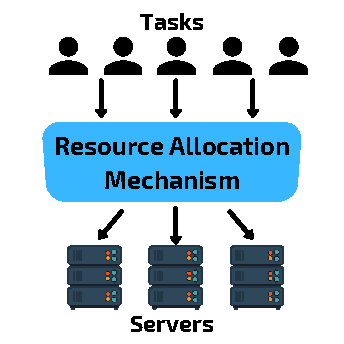
\includegraphics[width=\linewidth]{figs/system_model.pdf}
    \caption{System Model}
    \label{fig:system-model}
\end{wrapfigure}
A sketch of the system is shown in Fig.~\ref{fig:system-model}.
We assume that there are a set of servers $I = \{1,2,\ldots,\left|I\right|\}$, which could be accessed either through
cellular base stations or WiFi access points (APs). These servers have different types of limited resources:
storage for the code/data needed to run a task (e.g., measured in Gb), computation capacity in terms of CPU cycles per
time interval (e.g., measured in Ghz), and communication bandwidth to receive the data and to send back the results
of the task after execution per time interval (e.g., measured in Mbit). The servers are assumed to only consider these
attributes for resource allocation, however future work would wish to explore additional attributes like I/O memory
access per second, GPU usage, and more. The servers are also assumed to be heterogeneous in all their characteristics.
Formally, we denote the storage capacity of server $i$ with $S_i$, the computation capacity with $W_i$, and the
bandwidth capacity with $R_i$.

The system also contains a set $J = \{1,2,\ldots,\left| J \right|\}$, of different tasks that each require service from
one of the servers $I$. Each task has a monetary value, denoted $v_j$, representing the maximum price the owner is
willing to pay for the task to be computed. \\
In order to run a task, the server is required to load the appropriate code/data onto the server from a source, then to
compute the code of the task and to send back results to the user. Therefore, for each of these stages, we consider
separate speeds that the operations could occur at to enable the greatest flexibility for the server at each stage. \\
The storage size for the task $j$ is denoted as $s_j$ with the rate that the program is transferred to the server
as $s^{'}_j$. For a task to be computed successfully, it must fetch and execute instructions on a CPU. We consider the
total number of CPU cycles required for the program to be $w_j$, where the number of CPU cycles assigned to the task
per unit of time as $w^{'}_j$. Finally, after the task is run and the results obtained, the latter need to be sent back
to the user. The size of the results for task $j$ is denoted with $r_j$, and the bandwidth used to sent back results to
the user as $r^{'}_j$.

In order to force the server to complete the task with a reasonable time, each task sets a deadline, denoted by $d_j$,
representing the maximum amount of time for a task to be completed successfully within. This includes: the time
required to load the data/code onto the server, run it, and send back results to the user. We assume that there
is an \emph{all}-or-\emph{nothing} task execution reward scheme, meaning that the task value is awarded only if the
task is completed within its deadline.

\subsection{Optimisation problem}
\label{subsec:optimisation-problem}
Given the aforementioned assumptions and variables from the system model, an optimisation problem is constructed as
followed. This problem uses the additional variable $x_{i,j}$ to denote the allocation of a task $j$ that will run on
server $i$.

\begin{align}
    \max & \sum_{\forall j \in J} v_j \left(\sum_{\forall i \in I} x_{i,j}\right) \label{eq:objective} \\
    \mbox{s.t.} \nonumber \\
    & \sum_{\forall j \in J} s_j x_{i,j} \leq S_i, &~ \forall{i \in I} \label{eq:server-storage-constraint} \\
    & \sum_{\forall j \in J} w^{'}_j x_{i,j} \leq W_i, &~ \forall{i \in I} \label{eq:server-computation-constraint} \\
    & \sum_{\forall j \in J} (r^{'}_j + s^{'}_j) \cdot x_{i,j} \leq R_i, &~ \forall{i \in I} \label{eq:server-bandwidth-constraint} \\
    & \frac{s_j}{s^{'}_j} + \frac{w_j}{w^{'}_j} + \frac{r_j}{r^{'}_j} \leq d_j, &~ \forall{j \in J} \label{eq:task-deadline} \\
    & 0 < s^{'}_j, &~ \forall{j \in J} \label{eq:loading-speeds} \\
    & 0 < w^{'}_j, &~ \forall{j \in J} \label{eq:compute-speeds} \\
    & 0 < r^{'}_j, &~ \forall{j \in J} \label{eq:sending-speeds} \\
    & \sum_{\forall i \in I} x_{i,j} \leq 1, &~ \forall{j \in J} \label{eq:server-task-allocation} \\
    & x_{i,j} \in \{0, 1\}, &~ \forall{i \in I},\forall{j \in J} \label{eq:task-allocation}
\end{align}

The objective (eq.~\ref{eq:objective}) is to maximize the total value over all tasks (i.e.,\ social welfare) that
are completed within their deadline (eq.~\ref{eq:task-deadline}).
Constraints~\ref{eq:server-storage-constraint},~\ref{eq:server-computation-constraint}
and~\ref{eq:server-bandwidth-constraint}, prevent over allocation of server resources to allocated tasks.
For the server's storage capacity (constraint~\ref{eq:server-storage-constraint}), each server's storage must be less
than the allocated task's storage requirements. While for the server's computational capacity
(constraint~\ref{eq:server-computation-constraint}), the capacity is limited by a server's allocated tasks
compute resources ($w^{'}_j$). The server's bandwidth capacity (constraint~\ref{eq:server-bandwidth-constraint})
comprises of two parts: the first for loading of data/code of a task onto the server and the second for sending
back result to the user. \\
To force the task to the completed within its assigned deadline, constraint~\ref{eq:task-deadline} required the sum
of time taken for each stages of the task, completed in series, to be less than the deadline value.
Note that if a task is not allocated to any server, this constraints can be satisfied by choosing arbitrarily
resource speed as these resources do not use up any servers' resources in
constraint~\ref{eq:server-storage-constraint},~\ref{eq:server-computation-constraint}
or~\ref{eq:server-bandwidth-constraint}. \\
Constraints~\ref{eq:loading-speeds},~\ref{eq:compute-speeds},~\ref{eq:sending-speeds} enforce that the resource
speeds for each stage ($s^{'}_j$, $w^{'}_j$, and $r^{'}_j$) are all positive and finite.
Finally, as every task can only be served by at most one server, constraints~\ref{eq:server-task-allocation}
and~\ref{eq:task-allocation} enforce this.

This model focus on a single-shot setting where all tasks arrival at the same time to the system. To use this system
in practice where tasks arrival progressively over time, an allocation mechanism would repeat the allocation decisions
described here over regular time intervals. As a result, longer running tasks would reappearing in consecutive time
intervals.
In subsection~\ref{subsec:comparison-between-online-and-batched-resource-allocation}, we evaluate the effectiveness of
such a batching mechanism compared to online mechanisms. We leave a detailed study of online mechanisms to future work.
A probably advantage of such a system is the ability to dynamically change the resource allocation at each time step.

\subsection{Time Complexity}
\label{subsec:time-complexity}
As the optimisation problem as described in Subsection~\ref{subsec:optimisation-problem} is an extension of the
Knapsack problem, a well-studied problem in computer science that known to be NP-Hard. By transforming the problem into
a standard knapsack problem, the time complexity of the problem is also NP-Hard.
\begin{theorem}
    The optimisation problem in subsection~\ref{subsec:optimisation-problem} is NP-hard.
\end{theorem}
\begin{proof}
    The task resource elasticity~\ref{eq:task-deadline} can removed from the optimisation problem to simplify the model
    by setting the task resource speeds to a fixed value that satisfies the deadline constraint. This reduces the model
    to a 0--1 multidimensional knapsack problem~\cite{knapsackproblems_2004}, which is a generalization of a
    simple 0--1 knapsack problem. The latter is an NP-hard problem~\cite{knapsackproblems_2004}. Given this, it follows
    that the 0--1 multidimensional knapsack problem is also NP-hard. Since the optimization problem
    (Eqs.~\ref{eq:objective} -~\ref{eq:task-allocation}) is a generalization of a 0--1 multidimensional knapsack
    problem, it follows that it is NP-hard as well.
\end{proof}

\subsection{Example Problem Case}
\label{subsec:example-problem-case}
\begin{wrapfigure}{l}{0.5\linewidth}
    \centering
    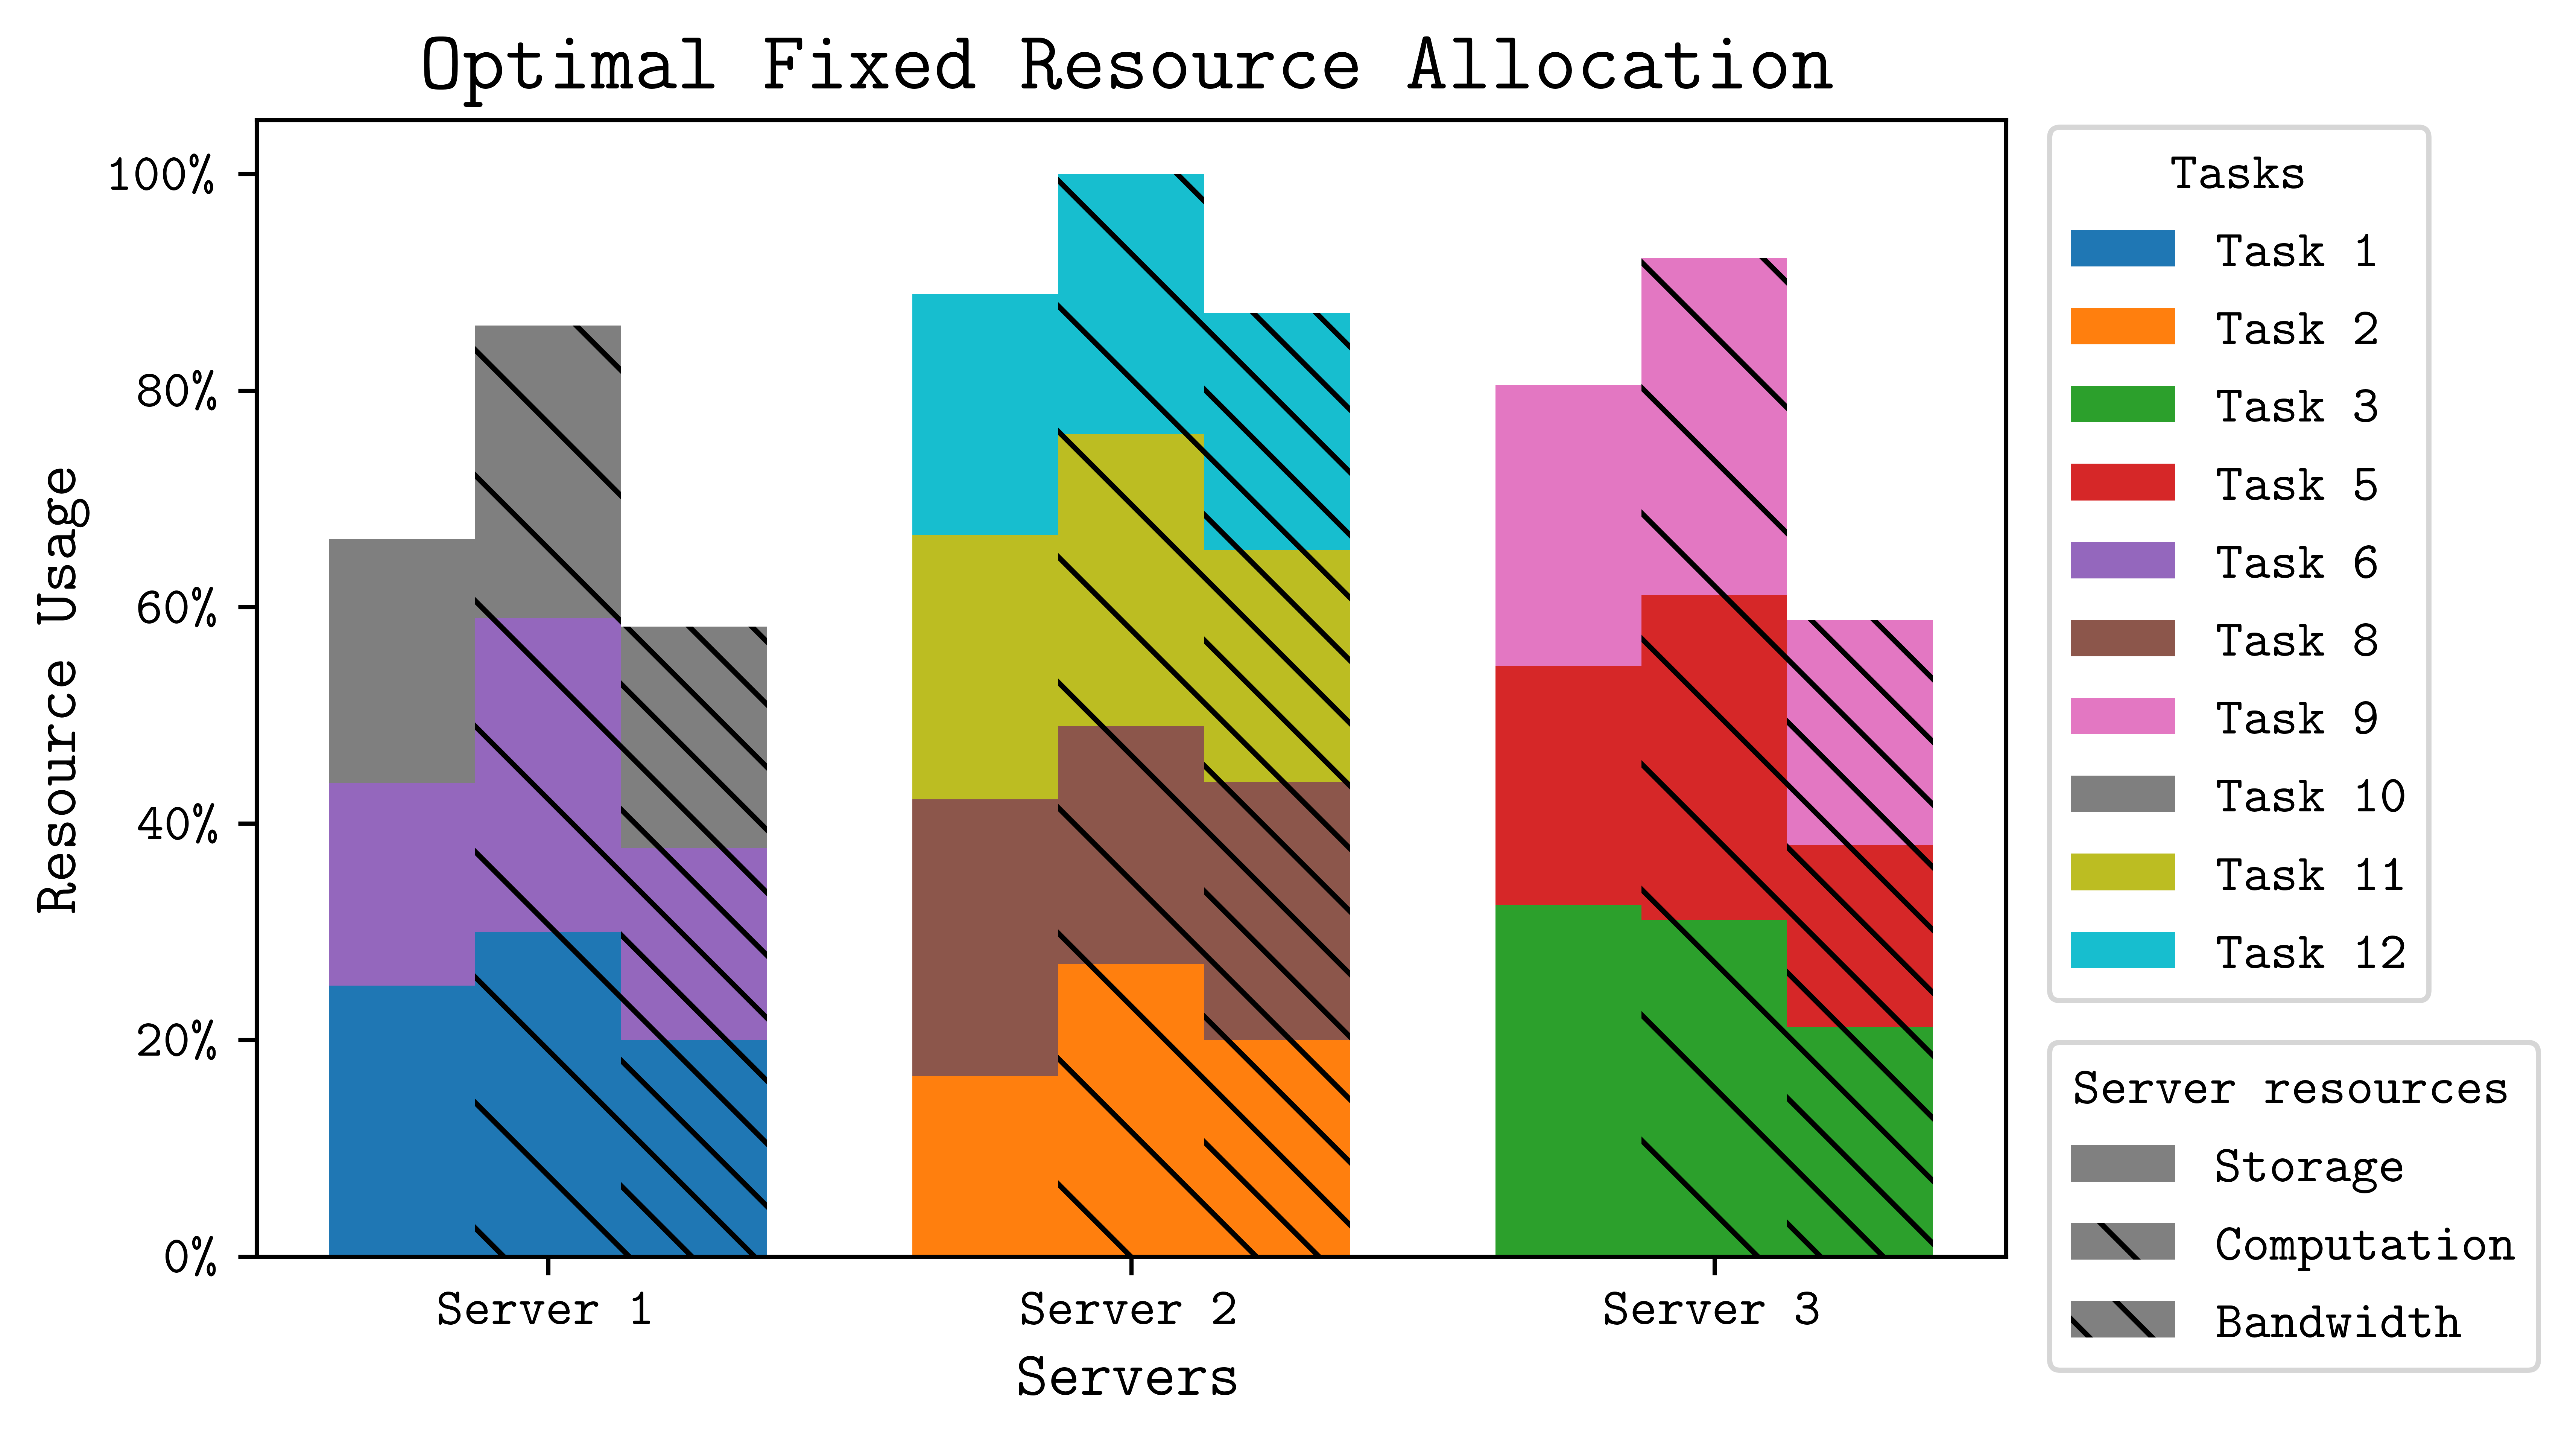
\includegraphics[width=\linewidth]{figs/allocation/optimal_fixed_resource_allocation.png}
    \caption{Optimal solution with fixed resource speeds}
    \label{fig:example-fixed-allocation}
\end{wrapfigure}
Before we propose our allocation mechanisms in the next section, we present an example case to illustrate
why elasticity is important. In this example, there are 12 potential tasks and 3 servers where the flexible solution
is able to achieve 18\% better social welfare compared to the fixed resource allocation solution.
The exact settings can be found in Appendix A with table~\ref{tab:example-tasks-properties}
for the task attributes and table~\ref{tab:example-servers-properties} for the server attributes. \\
The figures~\ref{fig:example-fixed-allocation} and~\ref{fig:example-flexible-allocation} represent each server as a
group of three bars, each relating to each server's resource type, with the percentage of resources used by a task
being the size of the bar.

\begin{figure}
    \centering
    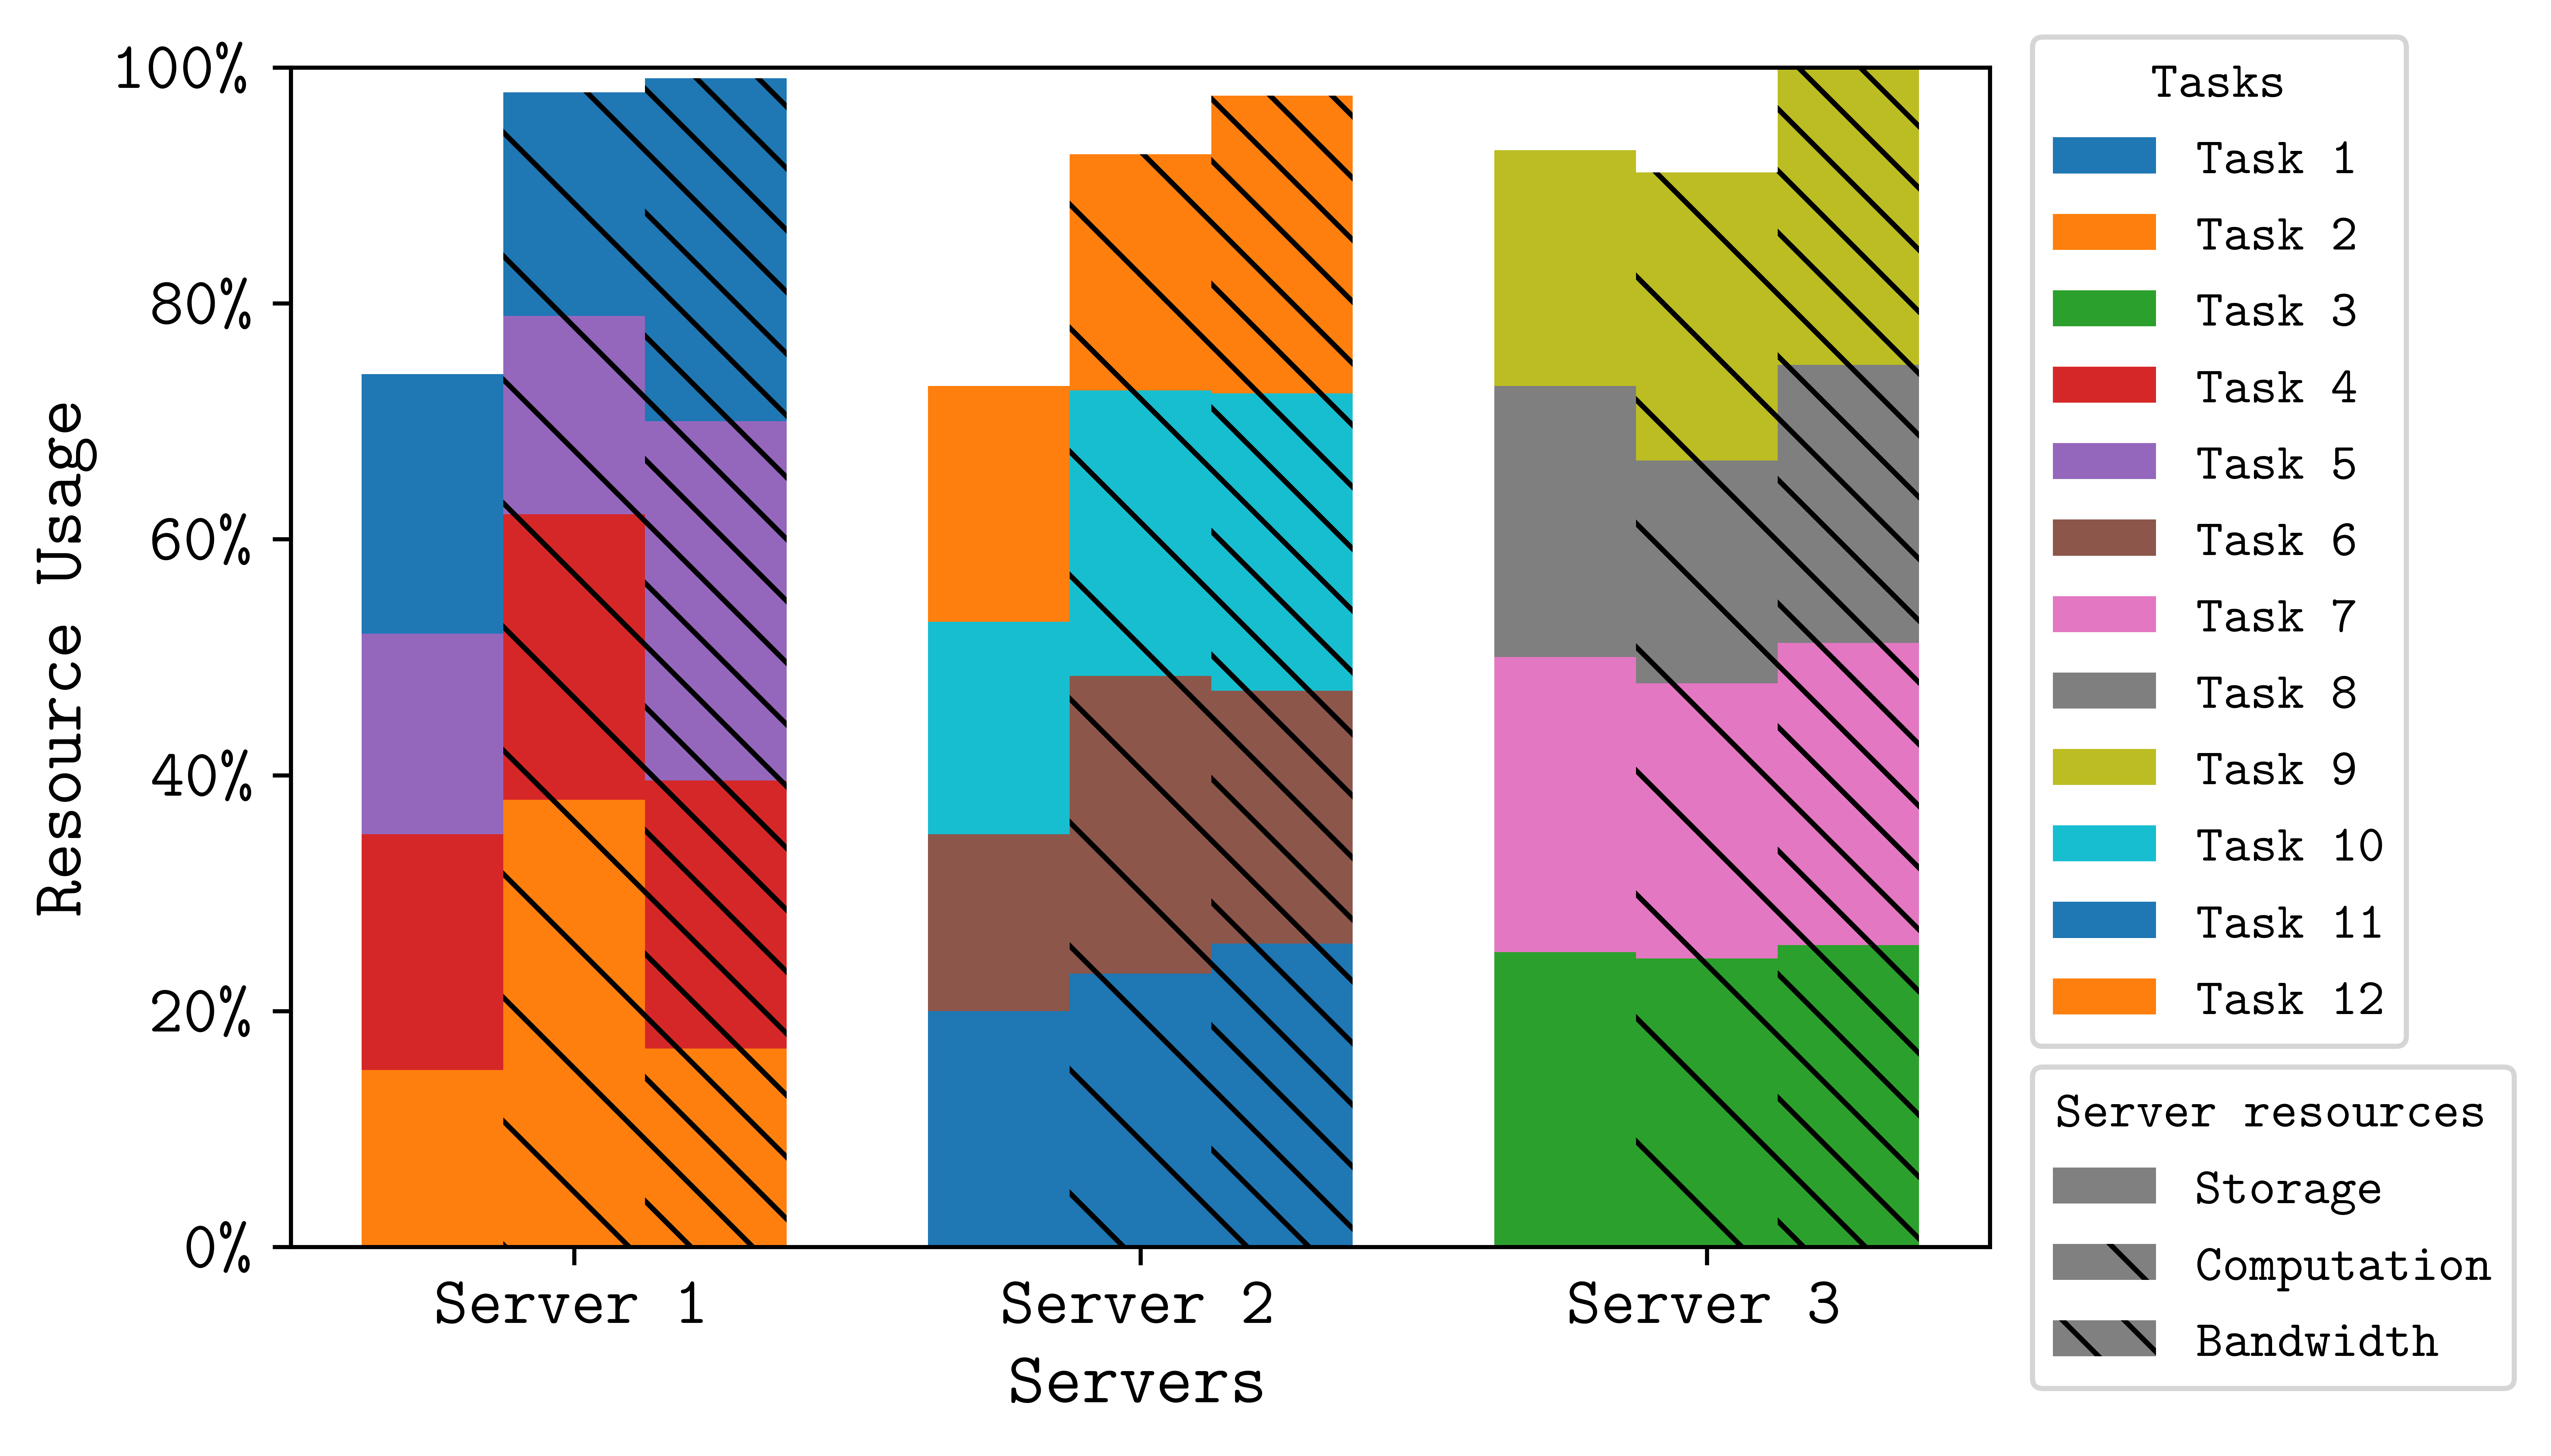
\includegraphics[width=0.5\linewidth]{figs/allocation/optimal_flexible_resource_allocation.png}
    \caption{Optimal solution with elastic resources speeds}
    \label{fig:example-flexible-allocation}
\end{figure}

Figure~\ref{fig:example-fixed-allocation} shows the best possible allocation if tasks have fixed resource speeds (which
were set by minimising the total amount of resources to be completed within the deadline). Here, only 9 of the tasks
are run, resulting in a total social welfare of 980 due to server 1 and 2's limited computational capacity and server
3' limited communication capacity.

In contrast to figure~\ref{fig:example-fixed-allocation}, Figure~\ref{fig:example-flexible-allocation} depicts the
optimal allocation if elastic resources are considered. Here, all the resources are used by the servers, whereas the
fixed example~\ref{fig:example-fixed-allocation} cant do this. In total, the elastic approach manages to schedule all
12 tasks within the resource constraints, achieving a total social welfare of 1200 (an 18\% improvement over the fixed
approach).
    \section{Flexible Resource Allocation Mechanisms}
\label{sec:flexible-resource-allocation-mechanisms}
As explained in the last Section, all previous research outlined in Section~\ref{sec:related-work} is incompatible
with our resource elastic optimisation problem in Section~\ref{sec:problem-formulation}. Therefore in this
section, we propose three mechanisms for solving this optimisation problem: an approximation algorithm and two
auction-based mechanisms. \\
The optimisation problem is a extended version of the knapsack problem, which is often solved using an dynamic
programming method that has pseudo-polynomial time complexity~\cite{toth1980dynamic}. The solution requires building
a table of items to bags allocation. For our problem, as the resource speeds must be considered at the same time, such
a solver can are infeasible due to both the space and time complexity required.

Because of this issue of allocating both tasks to a server and a server's resources to a task, this work proposes an
approximation algorithm where tasks are allocated to a server with resources in series not in parallel. The centralised
greedy algorithm (detailed in Subsection~\ref{subsec:greedy-algorithm}) ranks tasks that are each allocated to a server
with resources that at each stage uses a separate ranking function. This algorithm has a social welfare lower bound
of $\frac{1}{\left|J\right|}$, however in practice achieves close to the theoretical optimal while running with
polynomial time complexity.

As task users can be self-interested, they may report their task values or requirements strategically. Traditionally,
VCG~\cite{vickrey,Clarke,groves} is used for such systems due to its ability to use any optimisation problem to
calculate a task price. However, due to the difficulty of calculating the optimal allocation for this problem, VCG is
infeasible to use in this application. Therefore, to deal with self-interested users, we propose two auction-based
mechanisms. The first being an incentive-compatible auction using the centralised greedy algorithm
(Section~\ref{subsec:critical-value-auction}) and the second being a novel Decentralized Iterative
Auction (Section~\ref{subsec:decentralised-iterative-auction}) that does not require users to reveal the task value.

\subsection{Greedy Algorithm}
\label{subsec:greedy-algorithm}
To solve a knapsack problem, a greedy approximation algorithm is often used~\cite{sahni1975approximate}. We have
applied a similar approach to this problem specified in subsection~\ref{subsec:optimisation-problem}. As a result of
the elastic nature of task resources, an additional stage is required once a task has been allocated to a server in
order to determine the task's resource speeds.

\begin{wrapfigure}{r}{0.5\linewidth}
    \centering
    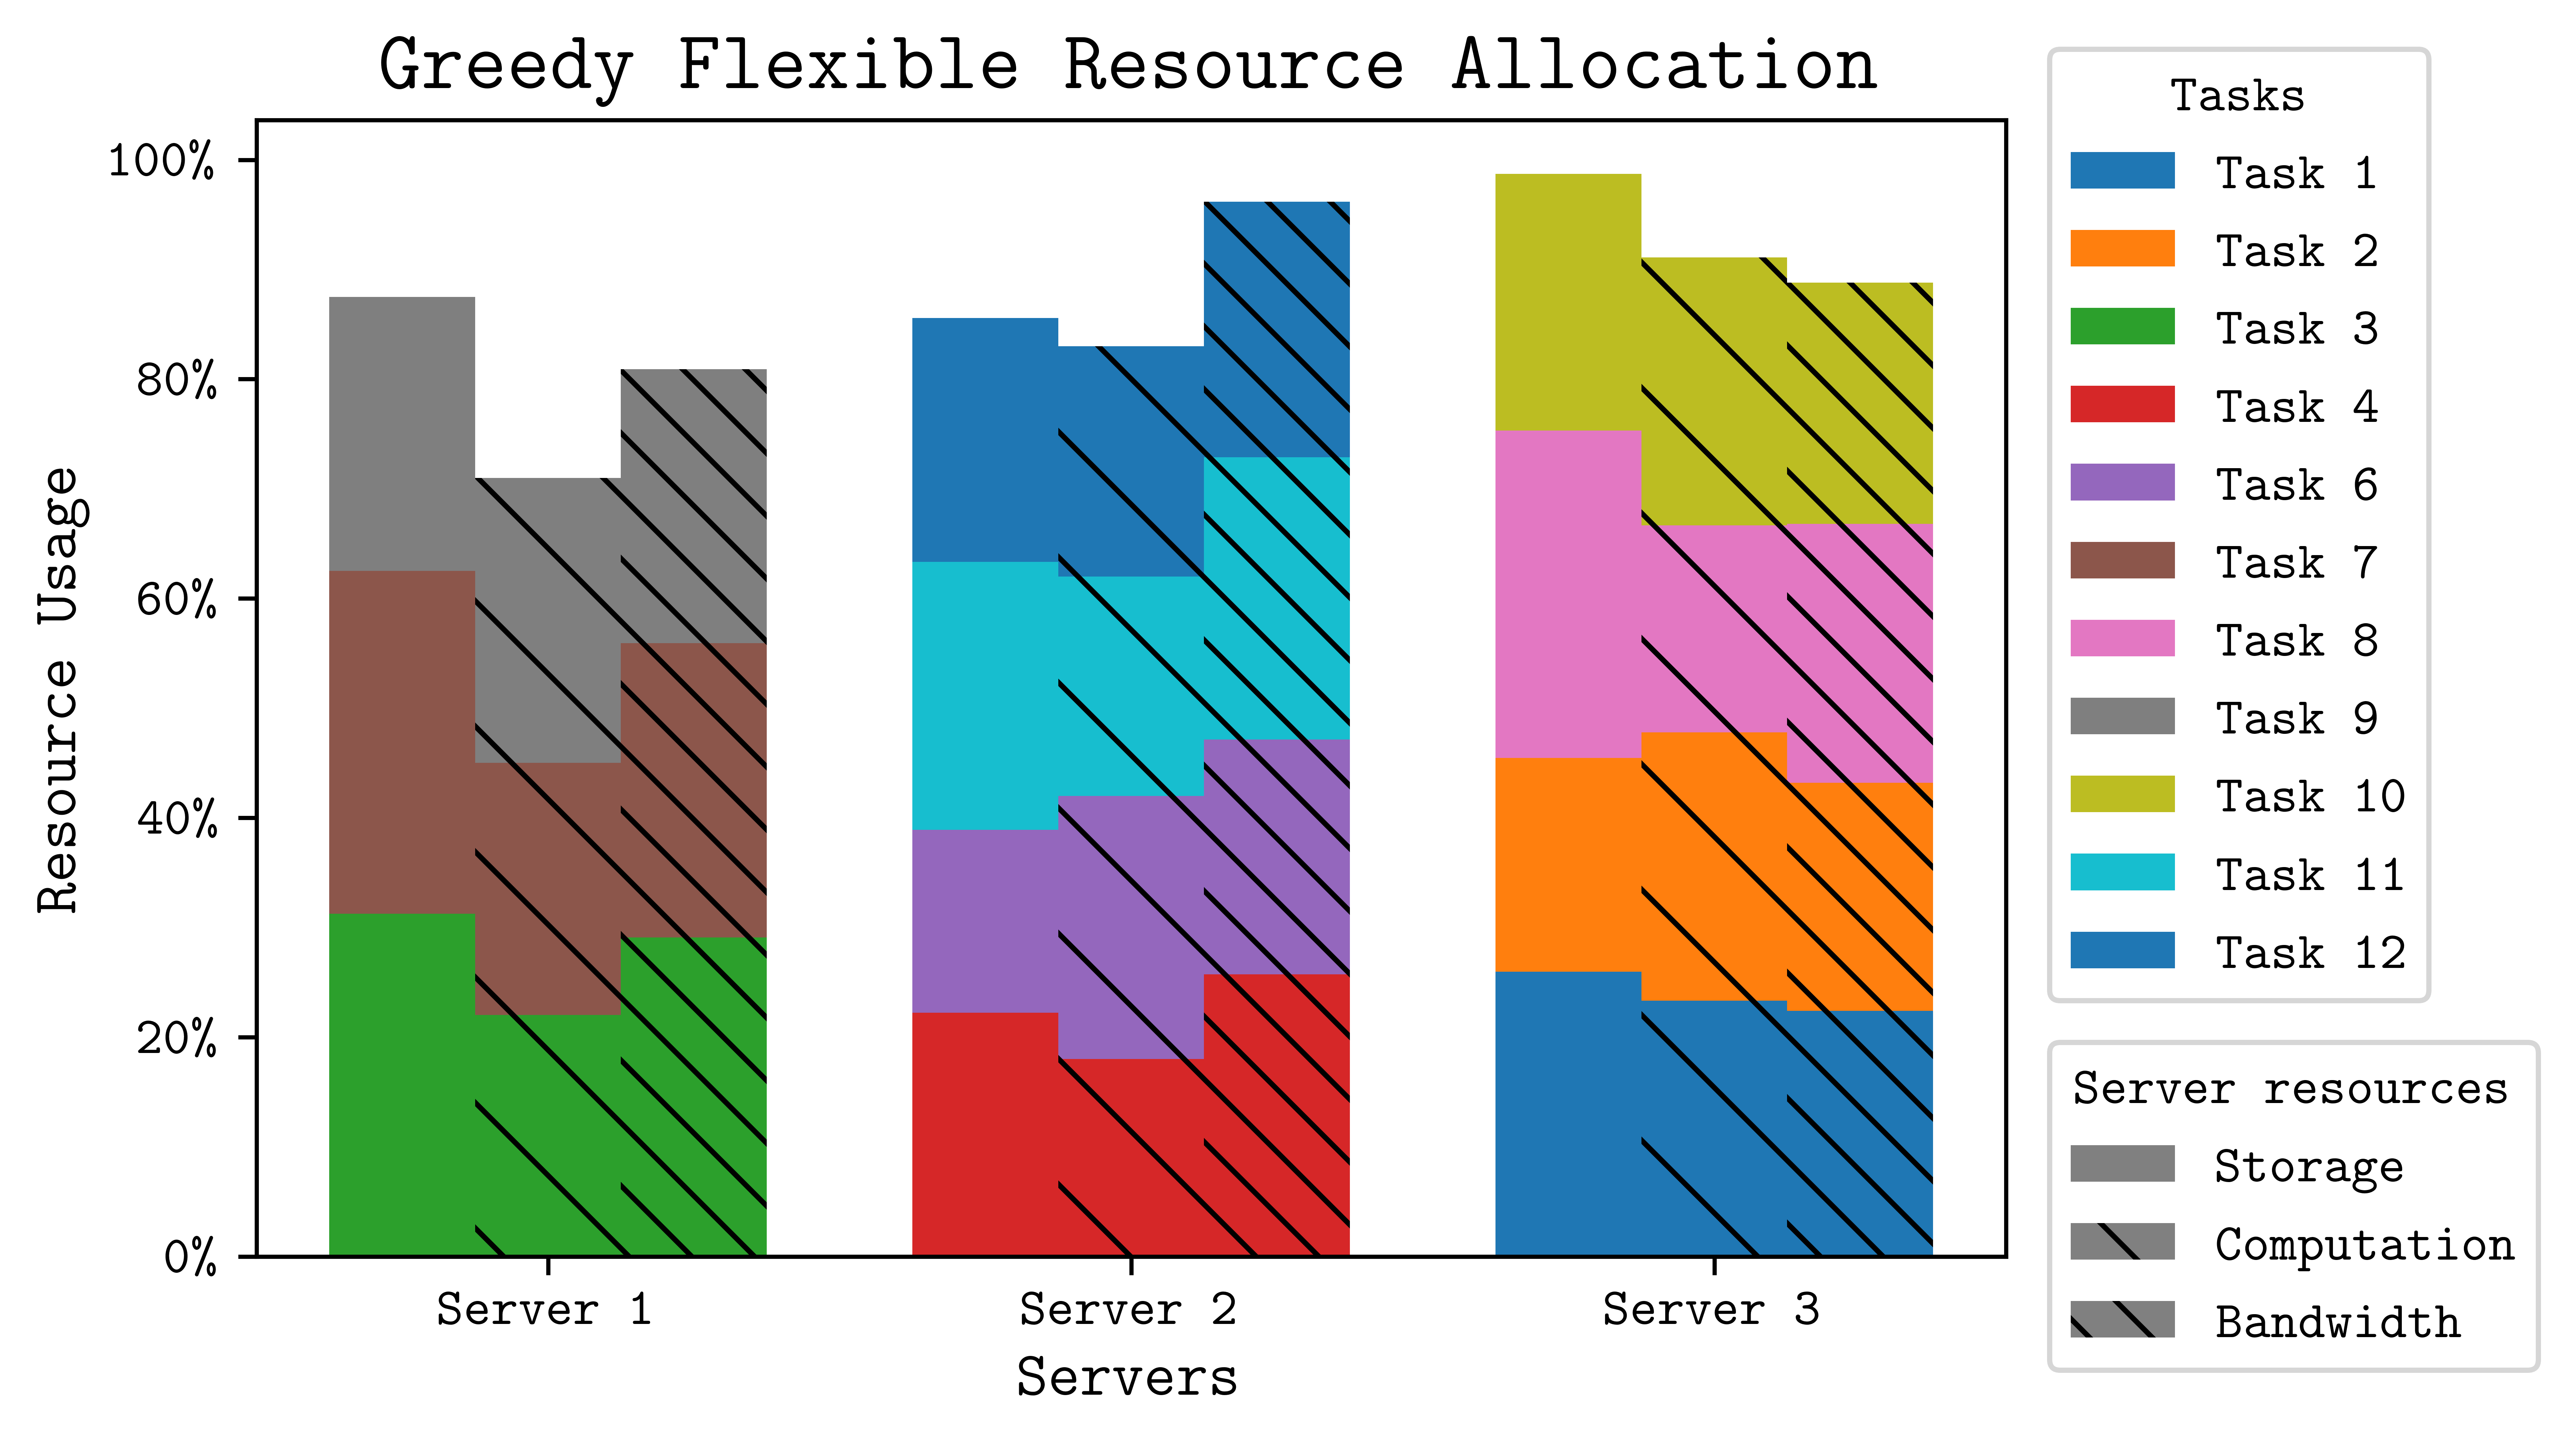
\includegraphics[width=\linewidth]{figs/allocation/greedy_flexible_resource_allocation.png}
    \caption{Example Greedy allocation using the model from table~\ref{tab:example-tasks-properties}
    and~\ref{tab:example-servers-properties}}
    \label{fig:example-greedy-allocation}
\end{wrapfigure}

More specifically, the greedy algorithm (algorithm~\ref{alg:greedy-algorithm}) has two stages; stage one sorts the list
of tasks based on the value density of each task calculated using task attributes: value, required resources and
deadline. The second stage uses the sorted list of tasks to iterate through applying two heuristics to select the
server based on available server resources and to allocate resources based on the available server resources and the
required resources of the task.

Using the example case from subsection~\ref{subsec:example-problem-case}, the greedy algorithm can complete 11/12 of
the tasks achieving XX\% more social welfare than the fixed solution. This is due to the algorithm being unable to % TODO
consider other tasks resource requirement while allocating resources. The greedy algorithm uses the value density
function, $\frac{v_j \cdot d_j}{s_j + w_j + r_j}$, for server selection,
$\text{argmin}_{\forall i \in I} S^{'}_i \cdot W^{'}_i \cdot R^{'}_i$ for task $j$ and servers $I$ and for the resource allocation
$\text{argmin}_{s^{'}_j, w^{'}_j, r^{'}_j} \left(\frac{w^{'}_j}{W^{'}_i}\right)^3 + \left(\frac{s^{'}_j + r^{'}_j}{R^{'}_i}\right)^3$
for task $j$ and server $i$.

\begin{algorithm}
    \caption{Pseudo code of Greedy Algorithm}
    \label{alg:greedy-algorithm}
    \begin{algorithmic}
        \REQUIRE $J$ is the set of tasks and $I$ is the set of servers
        \REQUIRE $S^{'}_i$, $W^{'}_i$ and $R^{'}_i$ is the available resources
            (storage, computation and bandwidth respectively) of server $i$
        \REQUIRE $v(j)$ is the value density function of task $j$
        \REQUIRE $s(j, I)$ is the server selection function of task $j$ and set of servers $I$ returning the best
            server, or $\emptyset$ if the task is not able to be run on any server
        \REQUIRE $r(j, i)$ is the resource allocation function of a task and server returning a tuple of the
            loading, compute and sending speeds
        \REQUIRE $\text{sort}(X, f)$ is a function that returns a sorted list of elements in descending order, based
            on a set of elements $X$ and a function for comparing elements $f$

        \STATE{$J^{'} \leftarrow sort(J, v)$}
        \FORALL{$j \in J^{'}$}
            \STATE{$i \leftarrow s(j, I)$}
            \IF{$i \neq \emptyset$}
                \STATE{$s^{'}_j, w^{'}_j, r^{'}_j \leftarrow \gamma(j, i)$}
                \STATE{$x_{i,j} \leftarrow 1$}
            \ENDIF
        \ENDFOR
    \end{algorithmic}
\end{algorithm}

\subsubsection{Greedy Lower Bound}
\label{subsubsec:greedy-lower-bound}
The lower bound of the algorithm is $\frac{1}{\left|J\right|}$ (where $\left|J\right|$ is the number of tasks) with
the task value as the value density function. This lower bound is not affected by the server selection policy or the
resource allocation policy. \\
However in testing, we found that the task value function is not the best value density heuristic as it does not
consider the effect of deadlines or the required resources of the task. In Section~\ref{sec:empirical-results}, we
considered a wide range of heuristics, showing the results of the best heuristics over a range of settings.

\begin{theorem}
    The lower bound of the greedy algorithm is $\frac{1}{n}$ of the optimal social welfare.
\end{theorem}
\begin{proof}
    Due to a task not considering other task's resource requirements when allocating resources then no matter the
    server selection or resource allocation function, it can't be guaranteed that subsequent tasks can be allocated to
    any server. As a result, the algorithm can be guaranteed to achieve at least $\frac{1}{n}$ of the optimal social
    welfare by sorting the tasks by task value ($v(j) = j_v$). Using this, the first task from the sorted task list
    will have the maximum task value meaning the lower bound of the algorithm is $\frac{1}{n}$ of the optimal social
    welfare.
\end{proof}

\subsubsection{Greedy Time Complexity}
\label{subsubsec:greedy-time-complexity}
Using the greedy algorithm (algorithm~\ref{alg:greedy-algorithm}), the time complexity is polynomial,
$O(\left|J\right| \left|I\right|)$.
\begin{theorem}
    Time complexity of the greedy algorithm is $O(\left|J\right| \left|I\right|)$, where $\left|J\right|$ is the number
    of tasks and $\left|I\right|$ is the number of servers. Assuming that the value density and resource allocation
    heuristics have constant time complexity and the server selection function is $O(\left|I\right|)$.
    %% TODO to check if the resource allocation heuristic is constant time complexity (KKT) probably wrong
\end{theorem}
\begin{proof}
    The time complexity of stage 1 of the algorithm is $O(\left|J\right| \log(\left|J\right|))$ due to sorting the
    tasks and stage 2 has complexity $O(\left|J\right| \left|I\right|)$ due to looping over all the tasks and
    applying the server selection and resource allocation heuristics. Therefore the overall time complexity is
    $O(\left|J\right| \left|I\right| + \left|J\right| \log(\left|J\right|) = O(\left|J\right| \left|I\right|)$.
\end{proof}

\subsection{Critical Value Auction}
\label{subsec:critical-value-auction}
Due to the problem case being non-cooperative, if the greedy algorithm was used to allocate resources such that the
value is the price paid. This would be open to manipulation and misreporting of task attributes like the value,
deadline or resource requirements. Therefore, in this section we propose an auction that is strategy-proof
(weakly dominant incentive compatible) so users have no incentive to misreport task attributes.

Single-Parameter domain auctions are extensively studied in mechanism design~\cite{nisan2007algorithmic_228} and are
used where an agent's valuation function can be represented as a single value. The task price is calculated by finding
the critical value, the minimum task price required for the task still allocated to any server. This has
been shown to be a strategy-proof~\cite{nisan2007algorithmic_229_230} auction making it a weakly dominant strategy for
all users to honestly reveal their task attributes.

\begin{algorithm}
    \caption{Pseudo code of the Critical Value Auction}
    \label{alg:critical-value-auction}
    \begin{algorithmic}
        \REQUIRE $J$ is the set of tasks and $I$ is the set of servers
        \REQUIRE $S^{'}_i$, $W^{'}_i$ and $R^{'}_i$ is the available resources
            (storage, computation and bandwidth respectively) of server $i$
        \REQUIRE $v(j)$ is the value density function of task $j$ with $v^{-1}$ being the inverse of the value density
            function making the value the subject of the function
        \REQUIRE $s(j, I)$ is the server selection function of task $j$ and set of servers $I$ returning the best
            server, or $\emptyset$ if the task is not able to be run on any server
        \REQUIRE $r(j, i)$ is the resource allocation function of a task and server returning a tuple of the
            loading, compute and sending speeds
        \REQUIRE $\text{sort}(X, f)$ is a function that returns a sorted list of elements in descending order, based
            on a set of elements $X$ and a function for comparing elements $f$
        \REQUIRE $\text{can\_allocate}(j, I)$ determines whether task $j$ can be allocated to any server $I$
        \REQUIRE $\text{Greedy}(J, I, v, s, r)$ is the greedy algorithm (subsection~\ref{subsec:greedy-algorithm}) with
            tasks $J$, servers $I$, value density $v$, server selection policy $s$, resource allocation policy $r$.

        \STATE{$\text{Greedy}(J, I, v, s, r)$}
        \FORALL{$j^{'} \in \{j \in J | \exists x_{j, i} \forall i \in I\}$}
            \FORALL{$j \in J$}
                \IF{$j^{'} \neq j$}
                    \STATE{$i \leftarrow s(j, I)$}
                    \IF{$i \neq \emptyset$}
                        \STATE{$s^{'}_j, w^{'}_j, r^{'}_j \leftarrow \gamma(j, i)$}
                    \ENDIF
                    \IF{$\neg \text{can\_allocate} (j^{'}, I)$}
                        \STATE{$p_{j^{'}} \leftarrow v^{-1}(v(j), j^{'})$}
                    \ENDIF
                \ENDIF
            \ENDFOR
        \ENDFOR
    \end{algorithmic}
\end{algorithm}

% TODO rewrite
The auction (algorithm~\ref{alg:critical-value-auction}) is implemented using the greedy algorithm from
section~\ref{subsec:greedy-algorithm} by finding an initial allocation using every task's reported value. Then for
each task that is allocated, the task price is equal to the critical value is found by finding the minimum value of the
task such that it is still allocated. \\
To find the minimum value is a two-step process of removing the task from the list of tasks then running the greedy
algorithm. However after each task is allocated, a check is done to see if the critical task could be allocated to any
server. This is a constant time complexity operation by assuming that the server would allocate all of its available
resources for the deadline constant (eq~\ref{eq:task-deadline}). If the task can't be allocated to any server then the
value density of last task allocated is equalled to the required value density of the critical task (this assumes that
in the sorted list, the critical task would appear ahead thus a minor amount could be add thus to guarantee the
critical task is above). Using the value density and the value density function, through finding the inverse of the
value density function, with regards to the task value allows the task critical value to be calculated.

\subsubsection{Critical Value Auction Time Complexity}
\label{subsubsec:critical-value-auction-time-complexity}
The time complexity of the auction is $O(\left|J\right| \left|J\right| \left|I\right|)$, the greedy
algorithm repeated $\left|J\right|$ due to calculating each task's critical value.
\begin{theorem}
    The time complexity of the critical value auction is $O(\left|J\right| \left|J\right| \left|I\right|)$.
\end{theorem}
\begin{proof}
    %% Todo to rewrite after algorithm made
    The auction uses the greedy algorithm (subsection~\ref{subsec:greedy-algorithm}), that has time complexity of
    $O(\left|J\right| \left|I\right|)$. For each task allocated by the greedy algorithm, the critical value must be
    found. To find the critical value of each task requires rerunning a modified greedy algorithm, such that after each
    task is allocated a check is done to see if the current task could be allocated to any server. This is done by
    repeating the server selection and resource allocation functions for each task (excluding the critical task) with
    time complexity, $O(\left|J\right| \left|I\right|)$, until the critical task can no longer be allocated to any
    server (a constant time function). The task's critical value is calculated in constant time function. As a result,
    the time complexity for calculating the critical value for an individual task is $O(\left|J\right| \left|I\right|)$.
    Thus, the overall time complexity is $O(\left|J\right| \left|J\right| \left|I\right|)$ due to the critical value
    being found for every task.
\end{proof}

\subsubsection{Demonstrating that the Critical Value Auction is Strategyproof}
\label{subsubsec:critical-value-auction-strategyproof}
In order that the auction is strategyproof, the value density function must be
monotonic~\cite{nisan2007algorithmic_229_230}. This ensures that if a task misreports any attributes, it will result
in the value density of the task decreasing, increasing the price payed. Therefore a value density function must be in
the form of $\frac{v_j \cdot d_j}{\alpha(s_j, w_j, r_j)}$ such it is monotonic decreasing if a task attribute is
misreported.
\begin{theorem}
    The value density function $\frac{v_j \cdot d_j}{\alpha(s_j, w_j, r_j)}$ is monotonic increasing for task $j$
    assuming the function $\alpha(s_j, w_j, r_j)$ is monotonic increasing for each variable.
\end{theorem}
\begin{proof}
    In order to misreport the task value and deadline, misreported values must be less than their true value. Therefore
    if the value or deadline are decreased then the value density will likewise decrease. \\
    The opposite is true for a task's required resources (storage, compute and result data), as the misreported value
    must be greater than the true value otherwise the task would not be able to be completed. Therefore as the $\alpha$
    function will increase as the resource requirements increase, the resulting value density will decrease. \\
    So in all cases, the overall value density will decrease if the owner doesn't accurately report a task's attribute,
    making the function monotonic.
\end{proof}

\subsection{Decentralised Iterative Auction}
\label{subsec:decentralised-iterative-auction}
In some applications of edge cloud computing, keeping the value of a task a secret is important, for example in
military-tactical networks. Therefore we propose a novel Decentralised Iterative Auction based on the pricing principle
of the VCG auction~\cite{vickrey,Clarke,groves}. VCG auction calculates the price of an item by finding the
difference in social welfare if the item exists and when it doesn't exist.

Our proposed novel auction uses the same principle, except in reverse by finding the difference between the current
server revenue and the revenue when the task is allocated with a price of zero. To cause the overall revenue and
server revenue to increase, a small value called the Price change variable is added to the task price.

Our auction uses this principle by iteratively letting a task advertise its requirements to all the servers, who
respond with their price to run the task. This price is equal to the server's current revenue minus the solution to the
problem in subsection~\ref{subsubsec:decentralised-iterative-problem} plus the price change variable. This is done to
ensure that the total server revenue increases by accepting the task. Once all of the servers have responded, the task
can compare the minimum server prices to its private evaluation. This allows the task to privately select the server
that it runs on (assumed to be the server with the lowest price) otherwise the task will stop advertising as it knows
that its evaluation is lower than the price of any server.

An additional heuristic is used as well to reduce the number of rounds required to find the revenue optima at setting
an initial price for a task. This is useful to account for the minimum costs of running the task. The heuristic
is referred to as the Initial Price which is set individually by each server.

The algorithm~\ref{alg:dia} is a centralised version of the auction. The auction runs iteratively till no task is left
so either the task can't be allocated to any server or is allocated to a server for a price. In this centralised version,
a random task is selected which is then advertised to all of the server who each solve the problem in
subsection~\ref{subsubsec:decentralised-iterative-problem} to calculate the task price. The minimum price returned by
$P(i, k)$ is compared to the task's reverse price (the maximum amount the task is willing to pay). If the price is less
than the task value then the task is allocated to the minimum price server and the task price set to the agreed price.
Otherwise the task is removed from the set of tasks to be allocated. In the process of allocating a task to a server
could result in some other tasks being deallocated from teh server. These deallocated tasks are then added back to the
set of tasks to be allocated to be selected again.

\begin{algorithm}
    \caption{Decentralised Iterative Auction}
    \label{alg:dia}
    \begin{algorithmic}
        \REQUIRE $I$ is the set of servers
        \REQUIRE $J$ is the set of unallocated tasks, that is initial the set of all tasks
        \REQUIRE $P(i, k)$ is the solution to the problem in section~\ref{subsubsec:decentralised-iterative-problem}
            using the server $i$ and new task $k$. The server's current tasks is known to itself and its current
            revenue from tasks so not passed as arguments.
        \REQUIRE $\leftarrow_R$ will randomly select an element from a set

        \WHILE{$|J| > 0$}
            \STATE{$j \leftarrow_R J$}
            \STATE{$p, i \leftarrow \min_{i \in I} P(i, j)$}
            \IF{$p \leq v_j$}
                \STATE{$p_j \leftarrow p$}
                \STATE{Allocate task $j$ to server $i$}
                \STATE{Add tasks deallocated from server $i$ back to $J$}
            \ENDIF
            \STATE{$J \leftarrow J \setminus \{j\}$}
        \ENDWHILE
    \end{algorithmic}
\end{algorithm}

\subsubsection{Server revenue optimisation problem}
\label{subsubsec:decentralised-iterative-problem}
To find the optimal revenue for a server $m$ given a new task $n^{'}$ and a set of currently allocated tasks $N$ has a
similar formulation to the optimisation problem in section~\ref{subsec:optimisation-problem}. Except with an additional
variable for the task price $p_n$ for each task $n$.

\begin{align}
    \max & \sum_{\forall n \in N} p_n x_n\label{eq:dia-objective}\\
    \mbox{s.t.} \nonumber \\
    & \sum_{\forall n \in N} s_n x_n + s_{n^{'}} \leq S_m,\label{eq:dia-server-storage-constraint}\\
    & \sum_{\forall n \in N} w^{'}_n x_n + w_{n^{'}} \leq W_m, \label{eq:dia-server-computation-constraint}\\
    & \sum_{\forall n \in N} (r^{'}_n + s^{'}_n) \cdot x_n + (r^{'}_{n^{'}} + s^{'}_{n^{'}}) \leq R_m, \label{eq:dia-server-communication-constraint}\\
    & \frac{s_n}{s^{'}_n} + \frac{w_n}{w^{'}_n} + \frac{r_n}{r^{'}_n} \leq d_n, &~ \forall n \in N \cup \{n^{'}\} \label{eq:dia-task-deadline}\\
    & 0 < s^{'}_n < \infty, &~ \forall{n \in N \cup \{n^{'}\}} \label{eq:dia-loading-speeds}\\
    & 0 < w^{'}_n < \infty, &~ \forall{n \in N \cup \{n^{'}\}} \label{eq:dia-compute-speeds}\\
    & 0 < r^{'}_n < \infty, &~ \forall{n \in N \cup \{n^{'}\}} \label{eq:dia-sending-speeds}\\
    & x_n \in \{0,1\} &~ \forall{n \in N} \label{eq:dia-task-allocation}
\end{align}

The objective (Eq.~\eqref{eq:dia-objective}) is to maximize the price of all currently allocated tasks (not including
the new task as the price is zero). The server resource capacity constraints
(Eqs.~\eqref{eq:dia-server-storage-constraint},~\eqref{eq:dia-server-computation-constraint}
and~\eqref{eq:dia-server-communication-constraint}) are similar to the constraints in the standard model set out in
section~\ref{subsec:optimisation-problem} except with the assumption that the task $n^{'}$ is running. The deadline and
non-negative resource speeds constraints (\ref{eq:dia-task-deadline},~\ref{eq:dia-loading-speeds}
,~\ref{eq:dia-compute-speeds} and~\ref{eq:dia-sending-speeds}) are all the same equation as the standard formulation
for all the tasks plus the new task. As this formulation only considers a single server, the task allocation constraint
is not considered.

\subsubsection{Decentralised Iterative Auction properties}
\label{subsubsec:decentralised-iterative-auction-properties}
For our proposed auction, we consider four important properties in auction theory.
\begin{itemize}
    \item Budget balanced - True. Since the auction can run without an auctioneer, the auction can be run in a
        decentralised system with no ''middlemen'' taking some money. This means that all revenue goes straight to
        the servers from the tasks.
    \item Individually Rational - True. As the server need to confirm with the task if it is willing to pay an amount
        to be allocated, the task can check this against its secret reserved price preventing the task from ever paying
        more than it is willing.
    \item Incentive Compatible - False. The ability for tasks to profit from misreport task attribute is difficult to
        numerous reason: a task's cannot determine the choices of other task for which server they will choose, the
        order task get priced in (this is random) and can't lie about their value as this information isn't
        revealed. Task's can misreport it's attributes to force other task's to make decisions that would otherwise
        result in the misreporting task from being deallocated from a server. For example, if a task misreports some
        attributes it may result in it being cheaper for another task to select a different server. This would mean
        that the misreported task would not being deallocated that would otherwise would be. However for large scale
        systems, intentionally misreporting such attribute is extremely difficult to profit from. This is empirically
        shown in subsection~\ref{subsec:possibility-of-misreporting-task-attributes-in-decentarlised-iterative-auction}.
    \item Economic efficiency - False. The allocation of task's to server is completely random until server becomes full,
        because of this, the initial allocation and the random selection of task's meaning that often task's result in a
        local maxima rather than the global maxima. As a result, the auction is not 100\% economically efficient
        however the local optima are often close to the global maxima as shown in
        subsection~\ref{subsec:evaluation-of-the-auction-mechanisms}.
\end{itemize}

While the auction is not incentive compatible and tasks do not pay the critical value, unlike the critical value
auction, task's do pay the minimal amount for the task to be allocated. This is different from the critical value for
two reasons: the critical value is not found through a deterministic process and the auction is not economically
efficient resulting in the global maxima always being found possibly resulting in the task paying a different price
each time the auction runs.

\subsection{Attributes of the proposed algorithms}
\label{subsec:attributes-of-proposed-algorithms}
In this paper, we have presented three mechanisms to solve the optimisation problem proposed in
section~\ref{subsec:optimisation-problem}. Table~\ref{tab:attributes_algorithms} considers a range of
important attributes of the proposed algorithm to allow easy comparison between the Greedy algorithm,
Critical Value auction and Decentralised Iterative auction.

\begin{table}[H]
    \begin{tabular}{|p{3cm}|c|c|c|}
        \hline
        \textbf{Attribute} & Greedy Algorithm & Critical Value Auction & Decentralised Iterative Auction \\ \hline
        Truthfulness & & Yes & No \\ \hline
        Optimality & No  & No & No \\ \hline
        Scalability & Yes & Yes & No \\ \hline
        Task information requirements from users & All & All & All except the task value \\ \hline
        Communication over heads & Low & Low & High \\ \hline
        Decentralisation & No  & No  & Yes \\ \hline
    \end{tabular}
    \caption{Attributes of the proposed algorithms: Greedy Algorithm, Critical Value Auction and the
    Decentralised Iterative auction}
    \label{tab:attributes_algorithms}
\end{table}

    \section{Empirical Results}
\label{sec:empirical-results}
To evaluate the algorithms presented in Section~\ref{sec:flexible-resource-allocation-mechanisms},
this section analyses the performance of both the greedy and auctions algorithms
(subsections~\ref{subsec:evaluation-of-the-greedy-algorithm} and~\ref{subsec:evaluation-of-the-auction-mechanisms}).
We investigate the effect of server heuristics on the Decentralised Iterative Auction
(subsection~\ref{subsec:effectiveness-of-decentralised-iterative-auction-heuristics}) and
the possibility of misreporting task attributes within the Decentralised Iterative Auction
(subsection~\ref{subsec:possibility-of-misreporting-task-attributes-in-decentarlised-iterative-auction}).
Finally we analyse the effectiveness of elastic resource allocation given server resource capacity ratios
(subsection~\ref{subsec:the-effective-of-elastic-resources-given-server-resource-capacity-ratio})
and the comparison between online and batched resource allocation methods
(subsection~\ref{subsec:comparison-between-online-and-batched-resource-allocation}).

Within Edge Cloud Computing, we have found no de facto standard for testing resource allocation algorithms and
those used in related work do not consider a deadline applicable for our work. Therefore we have generated synthetic
models for our servers and tasks. This is done using a handcraft Gaussian distribution for each attribute that can be
found in Appendix B\@.

In order to compare the results of the different algorithms, a branch and bound solution was implemented to solve
the optimisation problem, from subsection~\ref{subsec:optimisation-problem}. However due to the difficulty of
finding the optimal solution, this algorithm was only used in smaller settings were the optimal could be found within
a reasonable amount of time. \\
The settings chosen were 3 servers and 15 tasks, 6 servers and 30 tasks and 8 servers and 40 tasks where \~70\% of
tasks are allocated. \\
To compare to previous work that utilise a fixed resource requirement, each task's resource speeds were determined by
finding the minimum sum total of resource speeds according to the task deadline. This aims to give each task a
balanced amount of each resource making comparisons as fair as possible.

\subsection{Evaluation of the Greedy Algorithm}
\label{subsec:evaluation-of-the-greedy-algorithm}
In order to compare the greedy algorithm, the branch and bound solution above can be used to find the optimal solution
for both the flexible and fixed resource allocation methods. However as explained above, to use the time required we
are not able to use the solution for the larger problem setting (8 servers and 40 tasks). Therefore by modifying the
greedy algorithm to use a fixed resource allocation we are able to find an approximate solution for the fixed resource
allocation case in the large setting. \\
Along with this, a relaxed solution was implemented with the branch and bound algorithm containing just a single
server that combined all of the server capacities into one. The optimisation problem for it can be found in Appendix C\@.
This was used as the upper bound for the social welfare as the server is able to complete at least as much as all of the
servers individual as well as use the remaining resources of the servers to possible compute more tasks. \\
For the greedy algorithm, a wide range of possible functions were tested with the best found being - value density
function: \[\frac{v_j \cdot d_j}{s_j + w_j + r_j}\] server selection:
\[\text{argmin}_{\forall i \in I} S^{'}_i \cdot W^{'}_i \cdot R^{'}_i\] for task $j$ and servers $I$ and the resource allocation:
\[\text{argmin}_{s^{'}_j, w^{'}_j, r^{'}_j} \left(\frac{w^{'}_j}{W^{'}_i}\right)^3 + \left(\frac{s^{'}_j + r^{'}_j}{R^{'}_i}\right)^3\]
is task $j$ and server $i$.

\begin{figure}
    \centering
    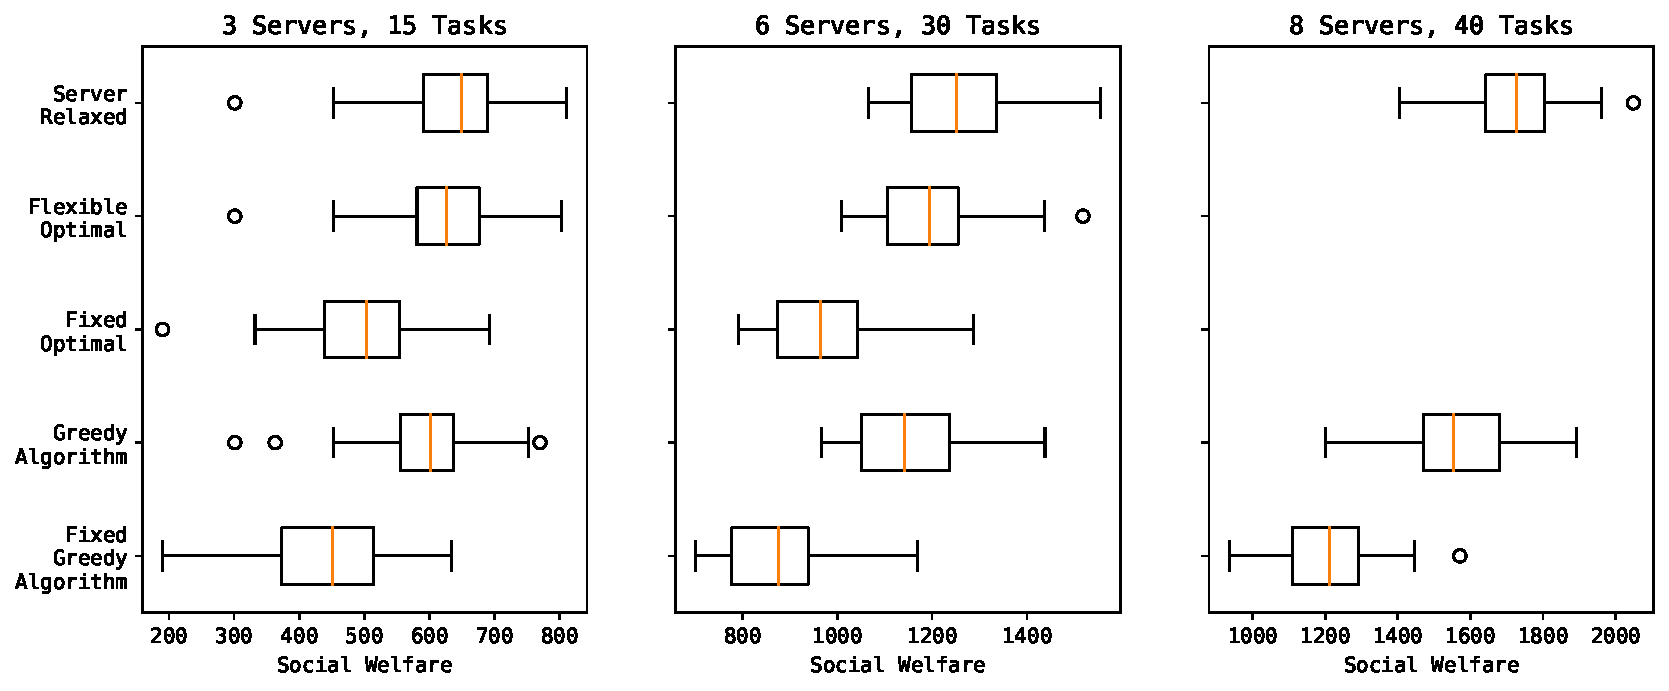
\includegraphics[width=\linewidth]{figs/greedy/multi_setting_social_welfare.pdf}
    \caption{Social welfare of the greedy algorithm, optimal flexible solution, optimal server relaxed solution,
             optimal fixed solution}
    \label{fig:greedy-algorithm-comparison}
\end{figure}
%% TODO Explain the results, percentage difference in social welfare with each algorithm and the difference
%% between the solutions for the optimal and approximation

\subsection{Evaluation of the Auction mechanisms}\label{subsec:evaluation-of-the-auction-mechanisms}
VCG, as explained in section~\ref{sec:flexible-resource-allocation-mechanisms}, is the traditional method of dealing
with self-interested users due to being incentive compatible. However, this requires solving the optimal solution
for each individual task making such a mechanism infeasible except for small setting. Because of this, VCG is used for
a comparison with the Critical Value Auction and Decentralised Iterative Auction in the smaller settings. \\
For the Critical Value Auction, the same function were used for the analyse of the greedy algorithm, in
subsection~\ref{subsec:evaluation-of-the-greedy-algorithm}. For the Decentralised Iterative Auction, the server
heuristics are a price change of 3 and an initial price of 25 for all servers. The reason for these heuristics over
others is explained in subsection~\ref{subsec:effectiveness-of-decentralised-iterative-auction-heuristics}.

\begin{figure}[h]
    \centering
    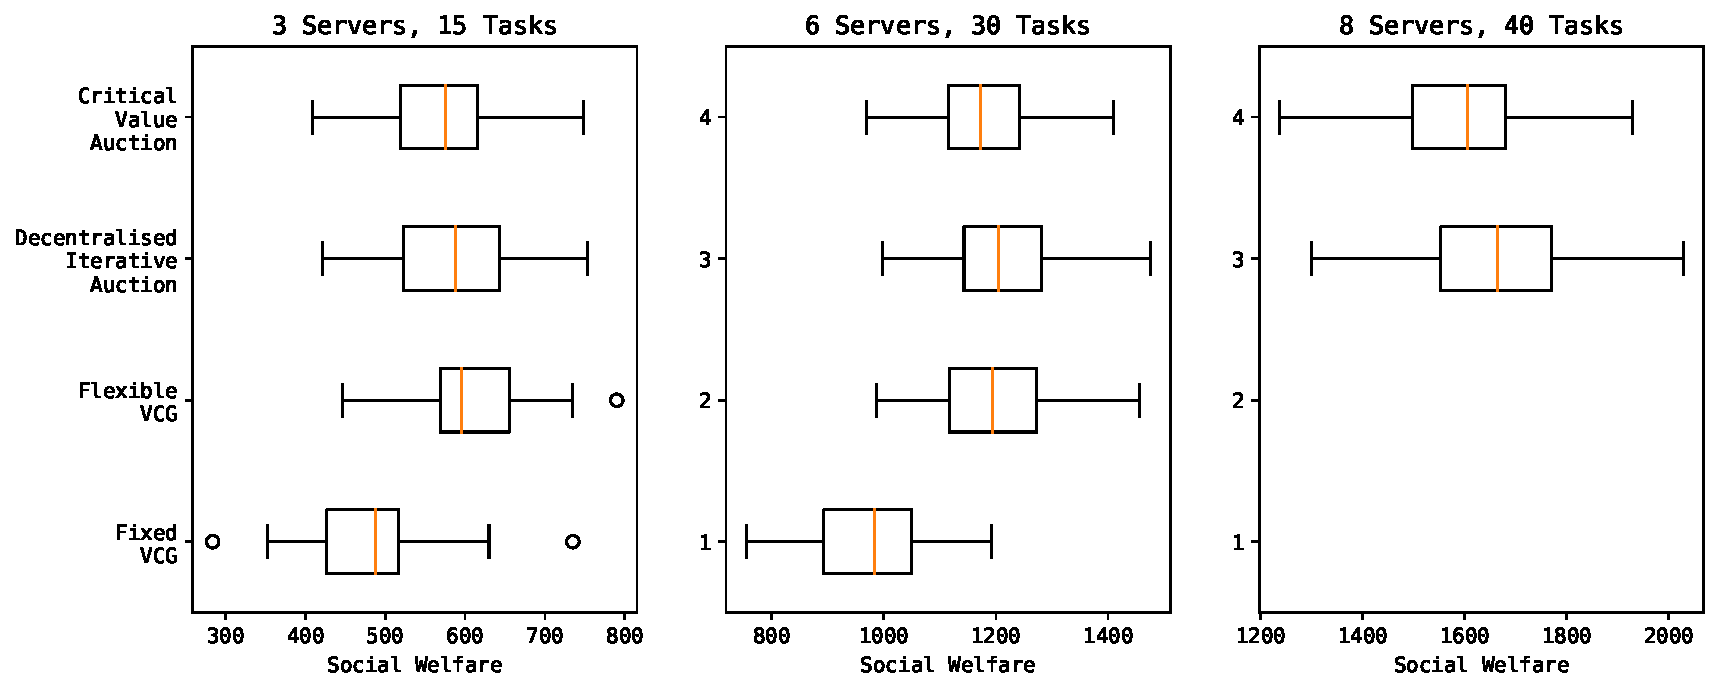
\includegraphics[width=\linewidth]{figs/auctions/multi_setting_social_welfare.pdf}
    \caption{Comparison of the social welfare for the auction mechanisms}
    \label{fig:auction-mechanisms-social-welfare}
\end{figure}

\begin{figure}[h]
    \centering
    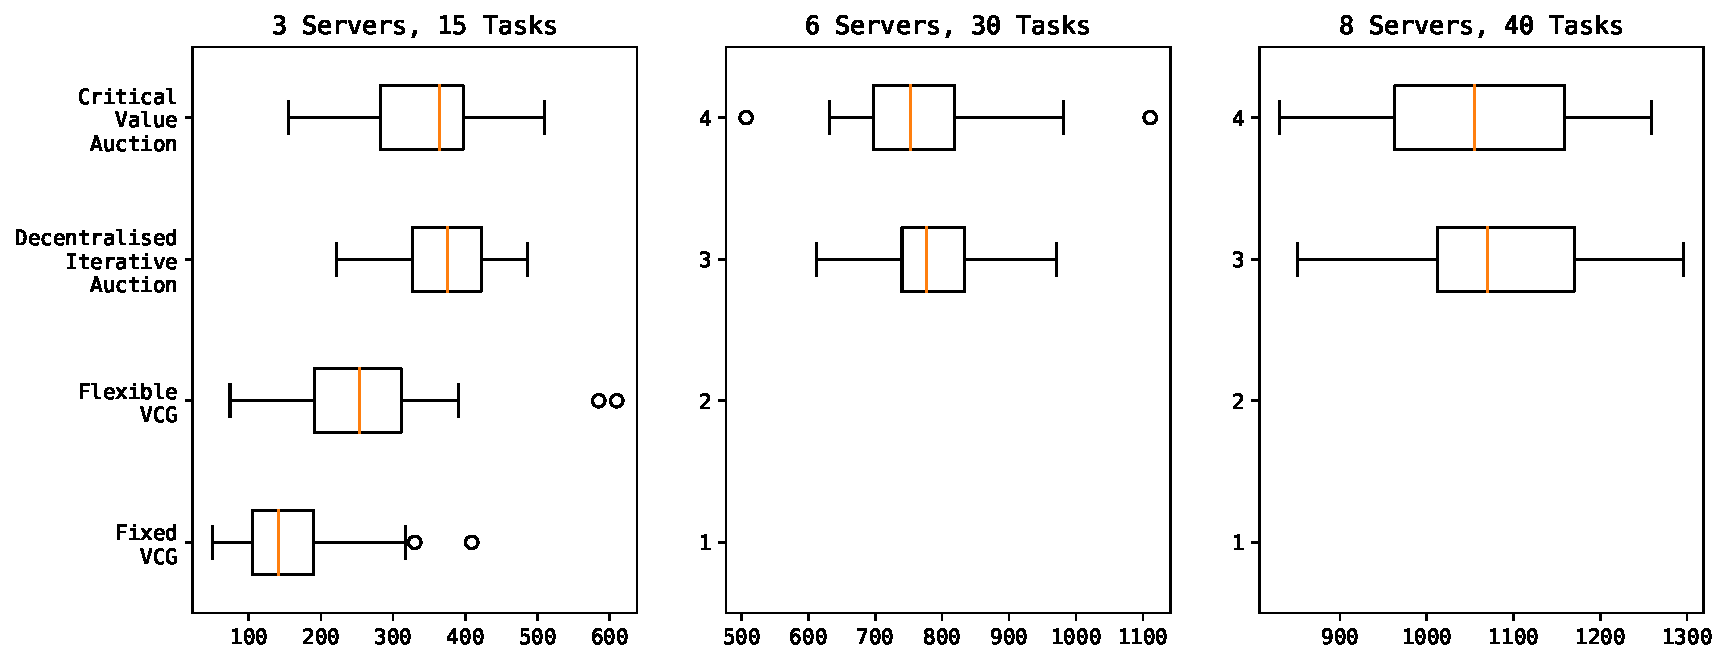
\includegraphics[width=\linewidth]{figs/auctions/multi_setting_revenue.pdf}
    \caption{Comparison of the social welfare for the auction mechanisms}
    \label{fig:auction-mechanisms-revenue}
\end{figure}

%% TODO explain the results, percentage difference in social welfare for the DIA and difference in revenue between
%%  algorithms

\subsection{Effectiveness of Decentralised Iterative Auction Heuristics}
\label{subsec:effectiveness-of-decentralised-iterative-auction-heuristics}
As explained in subsection~\ref{subsec:decentralised-iterative-auction}, the Decentralised Iterative Auction
calculates the price of task as the difference in revenue between the task being allocated (with a price of
zero) and not being allocated. To increase a server revenue, a server will increase the price by a value referred to as
the price change variable. \\
This is important as if a task has a value of 10 and the difference in revenue is 7 but the
price change is 4 then the resulting price is 11, above the task's value prevent it from being allocated. As a result,
the task won't be allocate to the server however if the price change was 3 then the task could have been allocated
resulting in the server's total revenue benefiting both the server and the task in question. \\
A second heuristic, the initial price variable, is used to speed up the auction and reduce the number of rounds by
aiming to set the price close to the task's actual value. This in turn reduces the number of rounds for the task price
to converge on the task value. However, a similar problem as the price change variable exists such that if the initial
price is greater than a tasks actual value then the task will never be allocated to a server. \\
Therefore the selection of price change and initial price can have a significant impact on the social welfare, revenue
and number of rounds the auction takes. As the mean value of tasks is 50 (see Appendix B),
the initial prices were set at 20, 25, 30, 35 and 40 while the price change variables were set at 1, 3, 5, 7, 10. These
values were chosen to allow for understanding the auction where value at both ends of the spectrum are used for both
variables, in order to see the effect on social welfare, revenue and number of rounds taken. For this case, we used
30 tasks and 6 servers.

\begin{figure}[h]
    \centering
    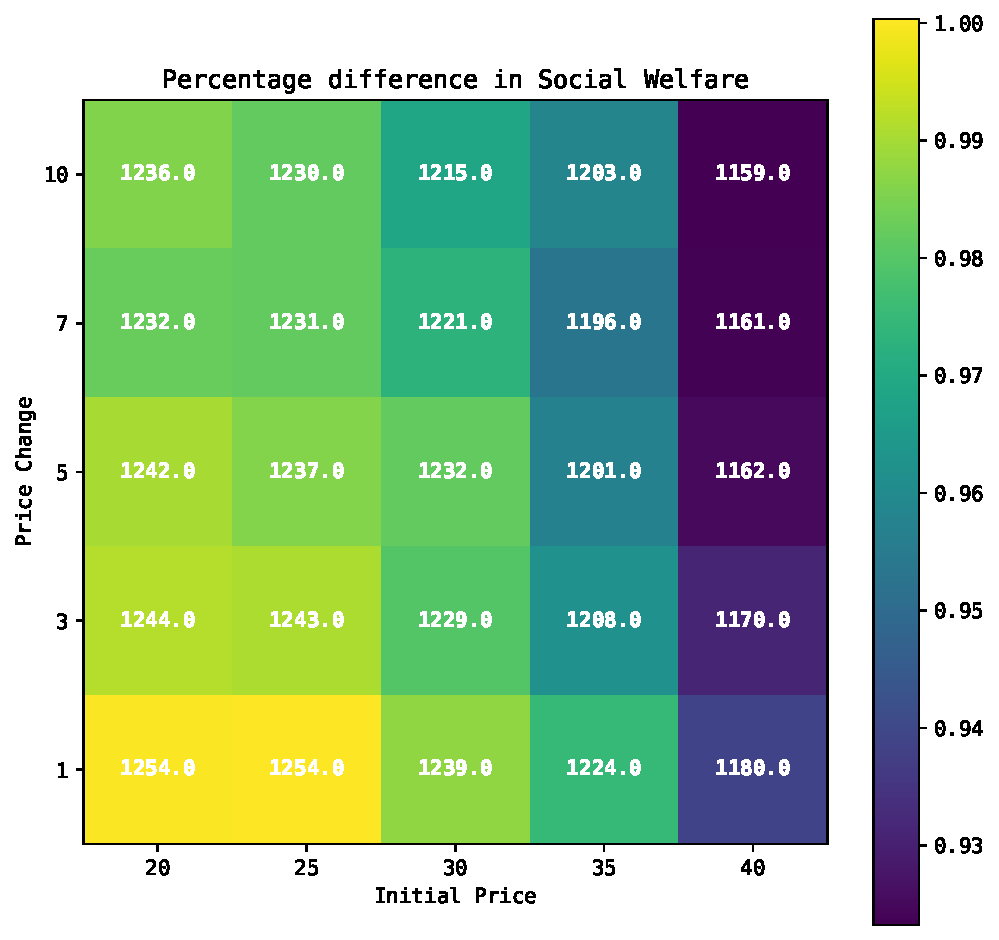
\includegraphics[width=0.45\linewidth]{figs/dia_heuristics/social_welfare_grid.pdf}
    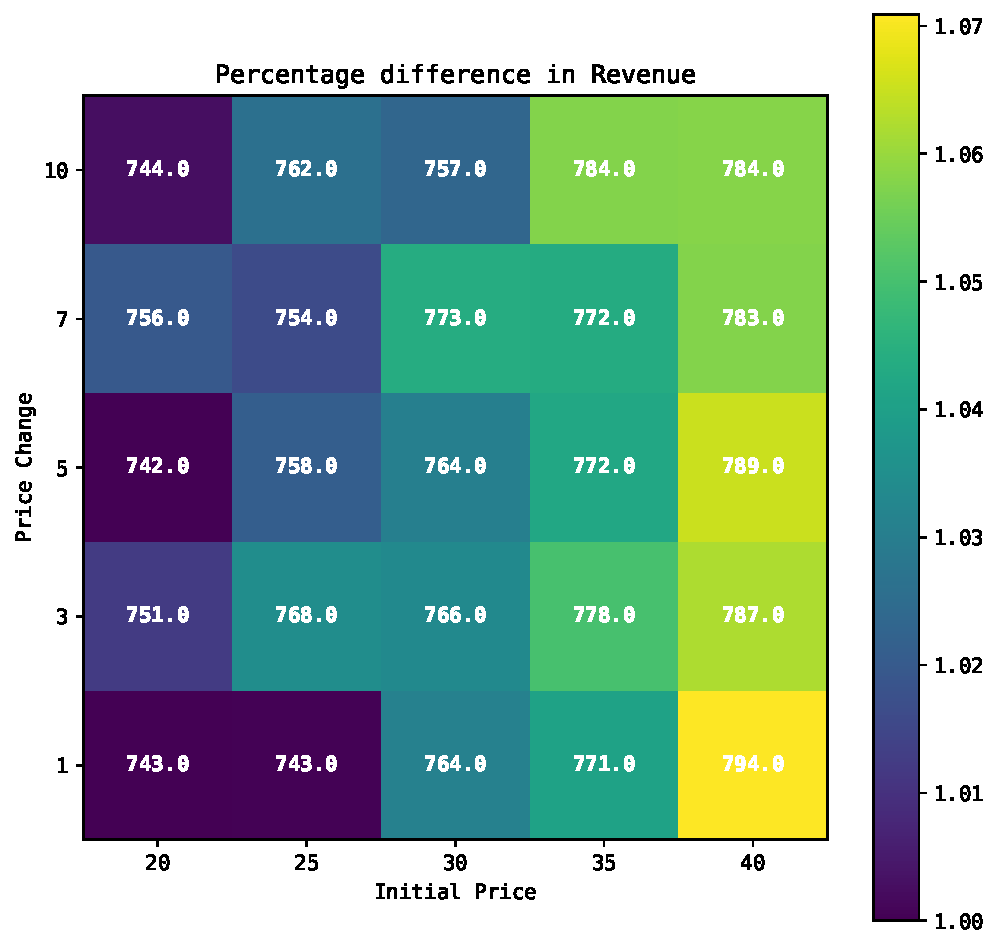
\includegraphics[width=0.45\linewidth]{figs/dia_heuristics/revenue_grid.pdf}
    \caption{Grid search of difference server price change and task initial cost effect on social welfare (left) and
             revenue (right)}
    \label{fig:dia-sw-rev-grid-search}
\end{figure}

%% TODO reread to make sure it makes sense
Figure~\ref{fig:dia-sw-rev-grid-search} maps a grid search of different price change and initial price values plotting
the social welfare on the left and the total revenue on the right. The value are normalised with the result of the
solution with a price change of 1 and initial price of 20. For the social welfare the percentage different between the
best case (price change of 1 and initial price of 20) to the worst results (price change of 10 and initial price of 40)
is only -7\% meaning that the auction is resilient to a range of price change and initial price values. \\
While interesting when measuring the revenue, the lowest revenue occurs for the case of price change of 1 and initial
price of 20. This is understandable as the system will arrive at a revenue local optima and for this case a majority of
tasks will pay their critical value however this also results in servers not gaining by forcing tasks by paying more
than they could have. However for the case with an initial price of 40, this forces tasks off the bat to pay a price of
40, in most cases more than their critical value.

Within the context of edge cloud computing, the number of rounds for the Decentralised Iterative Auction is important
to making it a feasible auction as the time taken is proportional to the number of rounds run.
Figure~\ref{fig:dia-rounds-grid-search} shows the number of rounds required on average for each heuristic. For the case where the
auction used the minimum heuristic values (price change of 1 and initial price of 20) that achieves the highest social
welfare comes at the close of requiring on average 400 rounds. This means that on average tasks require XX number %% TODO
of individual rounds to converge on a price. In comparison when the price change is set to 10 and the initial price is
kept at 20, the average number of rounds required is 5x less at 80.

This shows that the Decentralised Iterative Auction is an effective auction but has tradeoffs for server who must
choose whether to maximise social welfare, revenue or rounds as each requires a different selection of heuristics.

\begin{figure}[h]
    \centering
    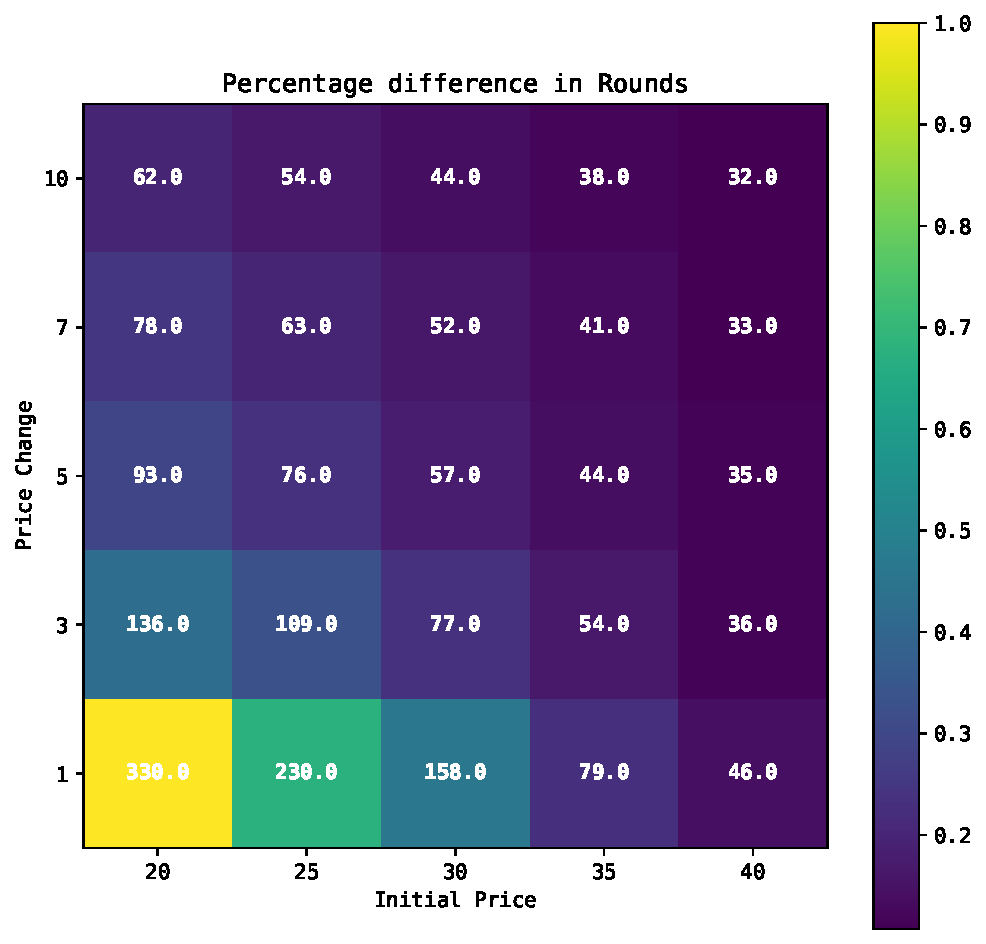
\includegraphics[width=0.45\linewidth]{figs/dia_heuristics/rounds_grid.pdf}
    \caption{Grid search of difference server price change and task initial cost effect on round count and number of
             task rounds}
    \label{fig:dia-rounds-grid-search}
\end{figure}

\subsection{The Possibility of Misreporting Task Attributes in Decentralised Iterative Auction}
\label{subsec:possibility-of-misreporting-task-attributes-in-decentarlised-iterative-auction}
In Subsection~\ref{subsec:decentralised-iterative-auction}, the Decentralised Iterative Auction was shown to be not
incentive compatible in specials cases however it is doubted that the ability for users to cheat more generally was
possible. Therefore, this problem was addressed by applying a grid search of task attributes and to randomly modify
individual tasks to investigate if tasks can pay less compared to if it didn't misreport.

For the random modification search, this was done by taking a random task and mutating each of the task's attributes.
% Todo Explain the grid search and random mutation results

\subsection{The Effective of Elastic Resources given Server Resource Capacity Ratio}
\label{subsec:the-effective-of-elastic-resources-given-server-resource-capacity-ratio}
The major advantage of using elastic resource allocation is to the control that it gives to servers. This becomes
increasing important if task requirements are unbalanced compared to server resource capacity. To measure the impact
of elastic resource allocation compared to fixed resource allocation, server computation and bandwidth capacities
are redistributed to different ratios in order to compare. The reason only the computation and bandwidth capacities
are modified is due to elasticity not affect the server's storage just its bandwidth and computation
(eq~\ref{eq:server-bandwidth-constraint} for loading and sending results and eq~\ref{eq:server-computation-constraint}
for computation results). \\
Server resources are redistributed using a percentage of the server's total (computation + bandwidth) resources.
This is shown as a ratio of server computation to bandwidth ratios in figures~\ref{fig:resource-ratio-social-welfare}
and~\ref{fig:resource-ratio-server-resource-usage}.

\begin{figure}[h]
    \centering
    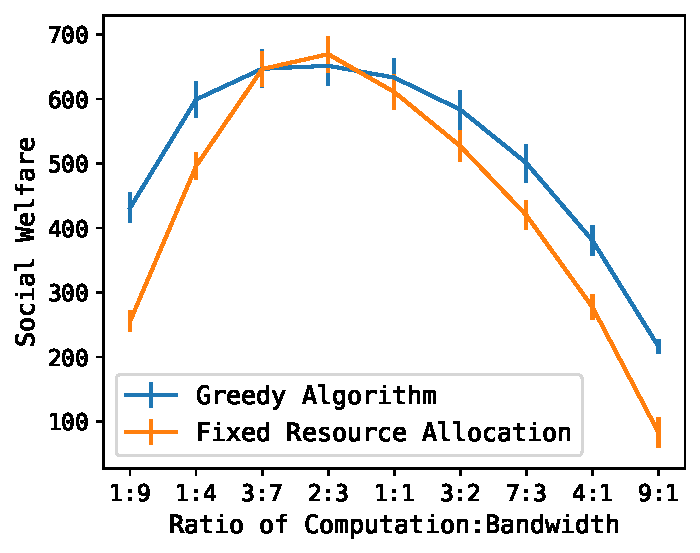
\includegraphics[width=0.45\linewidth]{figs/resource_ratio/social_welfare.pdf}
    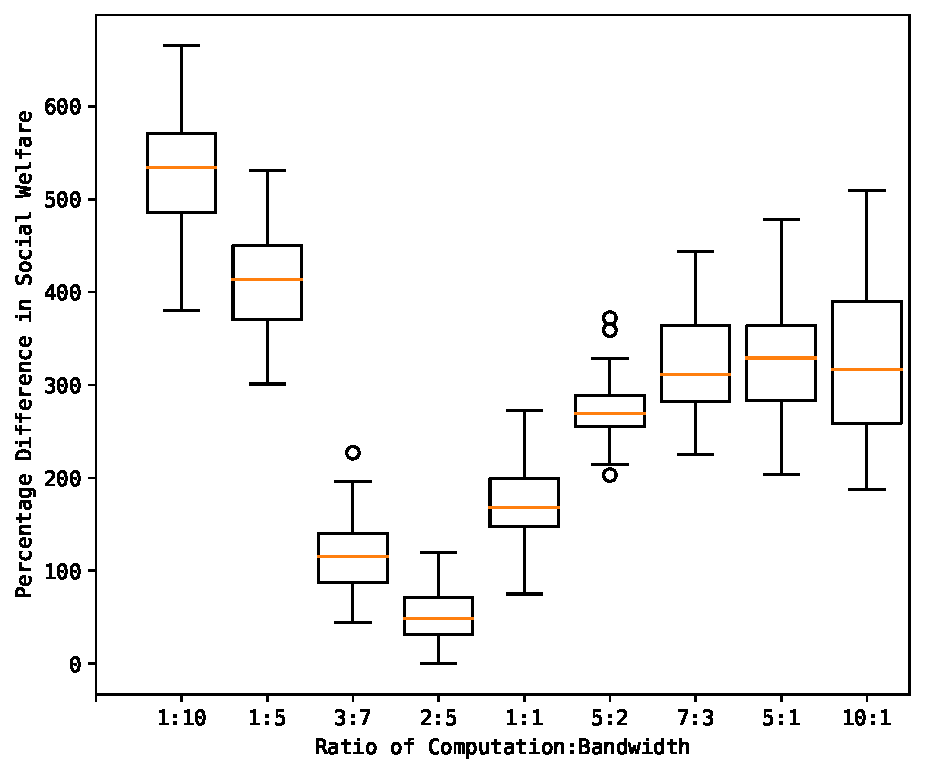
\includegraphics[width=0.45\linewidth]{figs/resource_ratio/social_welfare_difference.pdf}
    \caption{The effect of server resource ratios on average social welfare percentage and the social welfare difference}
    \label{fig:resource-ratio-social-welfare}
\end{figure}

Figure~\ref{fig:resource-ratio-social-welfare} is the combination of two graphs showing the same data. The left graph
shows the average social welfare achieved by the respective algorithms with different server resource ratios. As can be
seen on the figures at the ratio extremes, there is a significant difference in results between the flexible and fixed
resource allocation. This can be seen more clear by the right graph, that plots the difference in social welfare per
model with the error bars. \\
This observation is important for Edge Computing as nodes may have a large discrepancy in server resource capacity
due several reasons, i.e. a persistence task running over a long period of time, internet connection issues limiting
overall bandwidth, etc. For these cases, the elasticity of tasks has a significant boost to the number of tasks and
in social welfare in comparison to fixed resource allocation.

\begin{figure}[h]
    \centering
    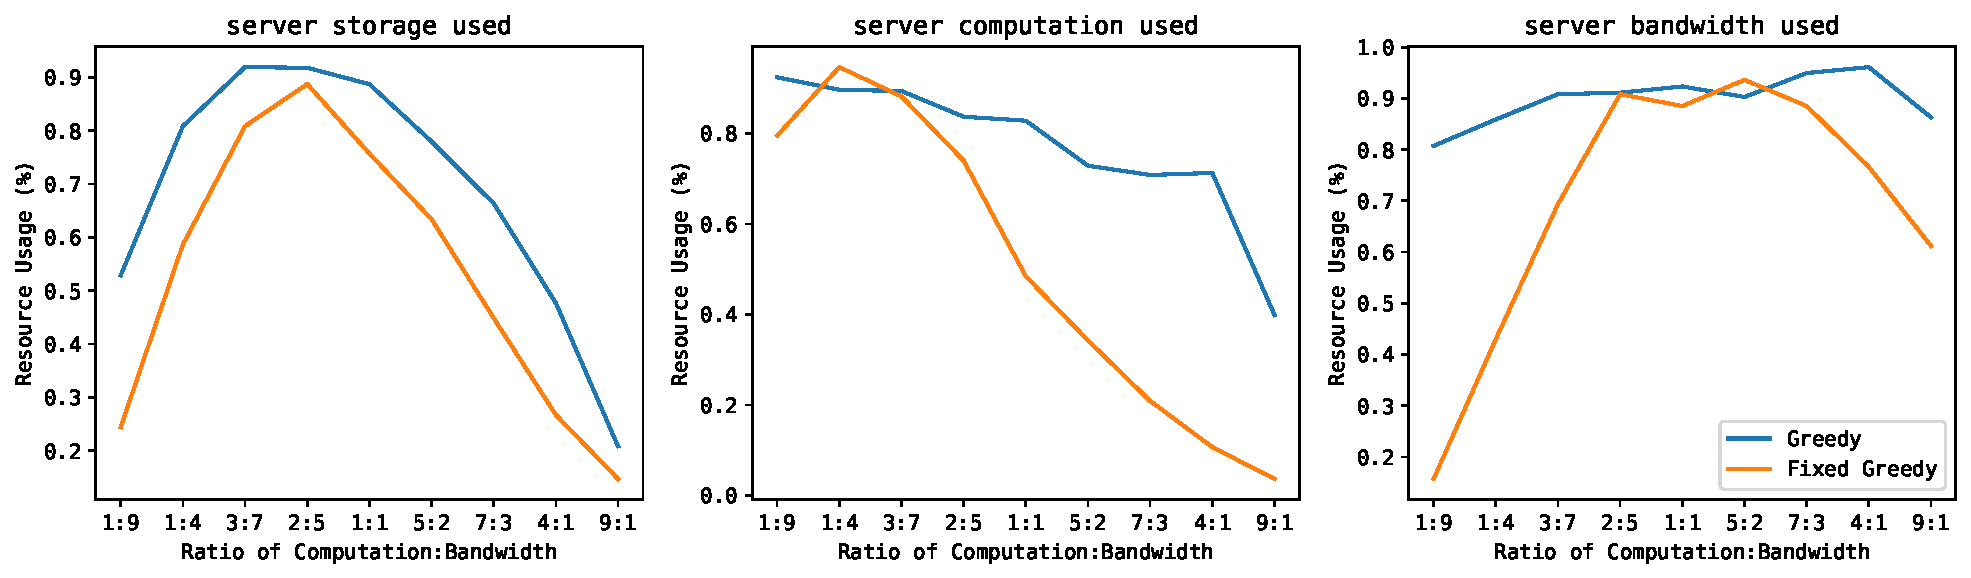
\includegraphics[width=\linewidth]{figs/resource_ratio/server_resource_usage.pdf}
    \caption{Server resource usage}
    \label{fig:resource-ratio-server-resource-usage}
\end{figure}

The effect of the redistribution of resources can be seen through the usage of resources by the servers per
each ratio in figure~\ref{fig:resource-ratio-server-resource-usage}. For cases where there is a large capacity of a
resource available, for elastic resource allocation these resources are able to be used to maximise the number of tasks
that can be run. This is particularly true of bandwidth as for a majority of the ratios, it is limiting factor for
allocating tasks.

\subsection{Comparison between Online and Batched Resource Allocation}
\label{subsec:comparison-between-online-and-batched-resource-allocation}
The purpose of this work has to be explore to use of elastic resource allocation in a static one-shot environment
meaning that all tasks arrive at the start, that are then allocated. However a problem exists with this formulation
that in reality, task do arrive over time. Section~\ref{sec:problem-formulation} proposed tasks are run in batches
overtime allowing no modifications to the algorithms proposed. This means that that as tasks arrive they are added to a
queue, such that when a new batch occurs, all of the tasks in the queue can be processed using the proposed algorithms
with no modifications. \\
Therefore choosing the right branch length is important as the more competition means better selection of tasks
increasing social welfare while the longer the branch length reduces the length of the task processing time. For the
Decentralised Iterative Auction, it has an advantage practically of being run in a batch as the auction doesn't need to
wait for all of the tasks to arrive compared to the Critical Value Auction. Therefore the auction can run during the
batch time frame with the task allocation at the end of the batch being the allocation.

We choose the batch lengths: 1, 2, 3, 4 because the mean length of a task is 10, any longer than this would result in
tasks on average tasks having to be computed in half their possible time. Plus, as can be seen in
figure~\ref{fig:batch-task-allocation}, the total social welfare decreases as the batch lengths increase investigating
longer batch lengths unwarranted.

\begin{figure}[h]
    \centering
    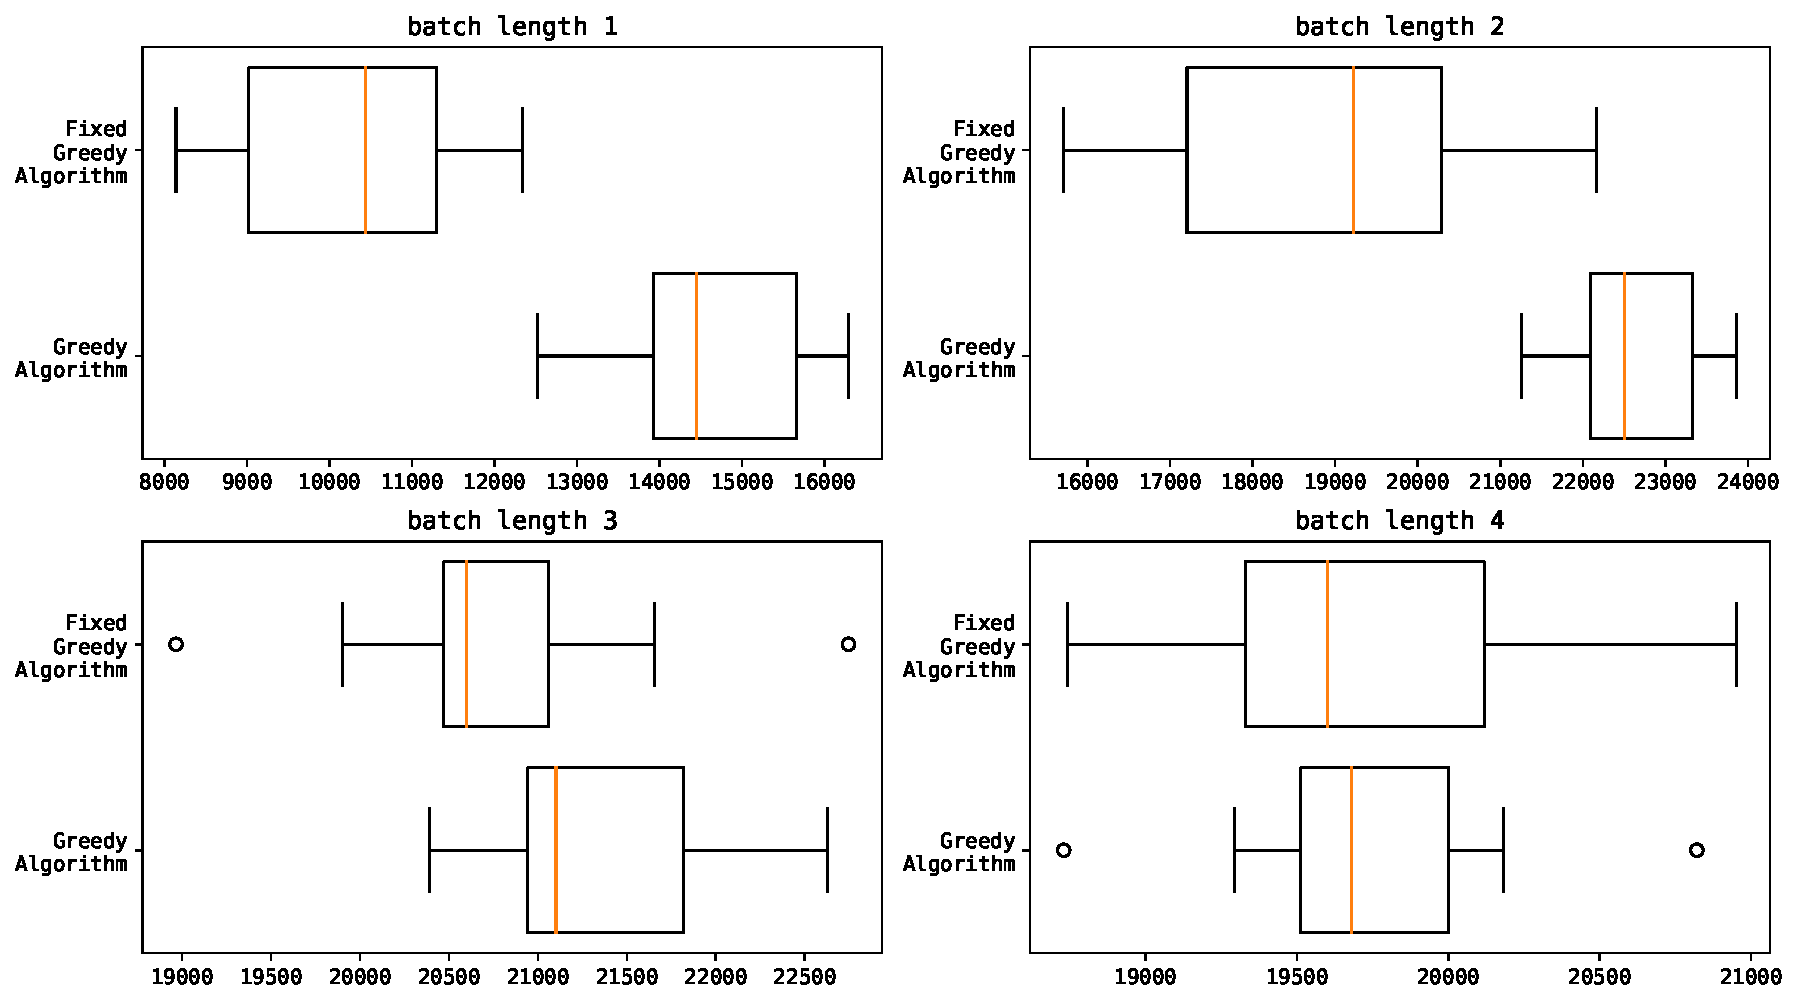
\includegraphics[width=\linewidth]{figs/online/online_batch_lengths.pdf}
    \caption{Online batch lengths}
    \label{fig:batch-task-allocation}
\end{figure}

%% TODO explain results
    \section{Conclusion and Future work}\label{sec:conclusion-and-future-work}
In this paper, we studied a resource allocation problem in edge clouds, where resources are elastic and can be
allocated to tasks at varying speeds to satisfy heterogeneous requirements and deadlines. To solve the problem,
we proposed a centralized greedy mechanism with a guaranteed performance bound, and a number of auction-based
mechanisms that also consider the elasticity of resources and limit the potential for strategic manipulation. We show
that explicitly taking advantage of resource elasticity leads to significantly better performance than current
approaches that assume fixed resources.

In future work, while this research considers online based mechanisms
(Subsection~\ref{subsec:comparison-between-online-and-batched-resource-allocation}), this was not the primary
environment these mechanisms were intended to occur within. Therefore additional research will focus primarily on this
online scenario.


    %% The next two lines define the bibliography style to be used, and
    %% the bibliography file.
    \bibliographystyle{ACM-Reference-Format}
    \bibliography{sections/references}

    %% If your work has an appendix, this is the place to put it.
    \appendix
    %! suppress = LabelConvention
\section*{Appendices}

\subsection*{Appendix A: Example problem case task and server attributes}
Within Subsection~\ref{subsec:example-problem-case} and~\ref{subsec:greedy-algorithm}, this example problem case is used
to demonstrate the effectiveness of elastic resource allocation compared to fixed resource allocation.
\begin{table}[h]
    \begin{minipage}{1.8in}
        \caption{Table of server attributes}
        \begin{tabular}{|c|c|c|c|}
            \hline
            Name     & $S_i$ & $W_i$ & $R_i$ \\ \hline
            Server 1 & 500   & 95    & 220   \\ \hline
            Server 2 & 500   & 95    & 210   \\ \hline
            Server 3 & 500   & 90    & 250   \\ \hline
        \end{tabular}
    \end{minipage}
    \begin{minipage}{3.5in}
        \caption{Table of task attributes. The columns ($s^{'}_j$, $w^{'}_j$, $r^{'}_j$) are fixed speeds which are not
        considered by the flexible resource allocation.}
        \begin{tabular}{|c|c|c|c|c|c|c|c|c|}
            \hline
            Name    & $v_j$ & $s_j$ & $w_j$ & $r_j$ & $d_j$ & $s^{'}_j$ & $w^{'}_j$ & $r^{'}_j$ \\ \hline
            Task 1  & 100   & 100   & 100   & 50    & 10    & 24        & 30        & 20        \\ \hline
            Task 2  & 90    & 75    & 125   & 40    & 10    & 23        & 27        & 19        \\ \hline
            Task 3  & 110   & 125   & 110   & 45    & 10    & 35        & 28        & 18        \\ \hline
            Task 4  & 75    & 100   & 75    & 60    & 10    & 25        & 25        & 20        \\ \hline
            Task 5  & 125   & 85    & 90    & 55    & 10    & 21        & 27        & 21        \\ \hline
            Task 6  & 100   & 75    & 120   & 40    & 10    & 20        & 29        & 19        \\ \hline
            Task 7  & 80    & 125   & 100   & 50    & 10    & 33        & 28        & 19        \\ \hline
            Task 8  & 110   & 115   & 75    & 55    & 10    & 30        & 22        & 20        \\ \hline
            Task 9  & 120   & 100   & 110   & 60    & 10    & 30        & 28        & 22        \\ \hline
            Task 10 & 90    & 90    & 120   & 40    & 10    & 27        & 27        & 18        \\ \hline
            Task 11 & 100   & 110   & 90    & 45    & 10    & 25        & 27        & 20        \\ \hline
            Task 12 & 100   & 100   & 80    & 55    & 10    & 24        & 24        & 22        \\ \hline
        \end{tabular}
    \end{minipage}
    \label{tab:example-tasks-server-properties}
\end{table}

\subsection*{Appendix B: Synthetic Model}
For the evaluation of the work in section~\ref{sec:empirical-results}, we used the following models. The left model
for the majority of the analyse with static one-shot cases and the right model for the analysing the online and batch
resource allocation methods.
\begin{table}[h]
    \begin{minipage}{2.8in}
        \begin{tabular}{|c|c|c|}
            \hline
            Attribute Name & Mean & Standard Deviation \\ \hline
            $v_j$          & 50   & 20                 \\ \hline
            $s_j$          & 100  & 15                 \\ \hline
            $w_j$          & 100  & 15                 \\ \hline
            $r_j$          & 50   & 10                 \\ \hline
            $d_j$          & 10   & 2                  \\ \hline
            $S_i$          & 450  & 50                 \\ \hline
            $W_i$          & 70   & 25                 \\ \hline
            $R_i$          & 290  & 45                 \\ \hline
        \end{tabular}
        \caption{Table of task and server attribute mean and standard deviations
        (used in section~\ref{sec:empirical-results})}
    \end{minipage}
    \begin{minipage}{2.8in}
        \begin{tabular}{|c|c|c|}
            \hline
            Attribute Name & Mean & Standard Deviation \\ \hline
            $v_j$          & 50   & 20                 \\ \hline
            $s_j$          & 100  & 15                 \\ \hline
            $w_j$          & 100  & 15                 \\ \hline
            $r_j$          & 50   & 10                 \\ \hline
            $d_j$          & 10   & 2                  \\ \hline
            $S_i$          & 400  & 40                 \\ \hline
            $W_i$          & 40   & 10                 \\ \hline
            $R_i$          & 150  & 20                 \\ \hline
        \end{tabular}
        \caption{Table of task and server attribute mean and standard deviations for the online work
        (used in subsection~\ref{subsec:comparison-between-online-and-batched-resource-allocation})}
    \end{minipage}
    \label{tab:synthetic-models}
\end{table}

\subsection*{Appendix C: Server Relaxed Optimisation Problem}
As an upper bound, a server relaxed version of the optimisation problem is used in
Subsection~\ref{subsec:evaluation-of-the-greedy-algorithm}. This is the optimisation problem solved by the branch and
bound solution.
\begin{align}
    \max & \sum_{\forall j \in J} v_j x_j \label{eq:relaxed-objective} \\
    \mbox{s.t.} \nonumber \\
    & \sum_{\forall j \in J} s_j x_j \leq S_i, \label{eq:relaxed-server-storage-constraint} \\
    & \sum_{\forall j \in J} w^{'}_j x_j \leq W_i,  \label{eq:relaxed-server-computation-constraint} \\
    & \sum_{\forall j \in J} (r^{'}_j + s^{'}_j) \cdot x_j \leq R_i \label{eq:relaxed-server-bandwidth-constraint} \\
    & \frac{s_j}{s^{'}_j} + \frac{w_j}{w^{'}_j} + \frac{r_j}{r^{'}_j} \leq d_j, &~ \forall{j \in J} \label{eq:relaxed-task-deadline} \\
    & 0 < s^{'}_j, &~ \forall{j \in J} \label{eq:relaxed-loading-speeds} \\
    & 0 < w^{'}_j, &~ \forall{j \in J} \label{eq:relaxed-compute-speeds} \\
    & 0 < r^{'}_j, &~ \forall{j \in J} \label{eq:relaxed-sending-speeds} \\
    & x_j \in \{0, 1\}, &~ \forall{j \in J} \label{eq:relaxed-task-allocation}
\end{align}
\end{document}
\endinput
%%
%% End of file `sample-manuscript.tex'.
